\cleardoublepage
\chapter{Resultater}
\label{chap:results} 

Dette kapittelet inneholder en presentasjon av prototypen gruppen har utviklet. Her beskrives også gjennomførte evalueringer av arbeidet, selve produksjonen og hvordan dette ble gjennomført, hvordan resultatet ble og det presenteres tester og vurderinger av prototypen og konseptet fra studenter, organisasjoner, fagpersoner og oppdragsgiver.

\section{Presentasjon av prototype}
\label{section:presentasjon-produkt}
Innhold beskrevet i kapittel~\ref{chap:method} resulterte i en navigerbar prototype utviklet i Adobe XD. Prosjektet inneholder 42 artboards med skisser laget av prosjektgruppen. Mange av disse skissene viser kun forskjellige valgmuligheter for samme funksjon og er derfor ikke gagnlig å presentere i oppgaven. For å kunne vise skissene for alle de forskjellige sidene til tjenesten i bildeformat ble det valgt ut 20 skisser som alle ligger vedlagt i tillegg~\ref{vedlegg:skisser3}. Fem av disse skissene blir også presentert videre i delkapittel~\ref{section:presentasjon-produkt}.

Sammen med {\em anbefalinger for utvikling og videre arbeid} beskrevet i delkapittel~\ref{section:anbefaling-videre-utvikling} og andre retningslinjer gitt i dette dokumentet, leveres prototypen til oppdragsgiver som et grunnlag for videre utvikling med instruksjoner og anbefalinger om hvordan formålet med tjenesten kan oppfylles.

\subsection{Minimalisme og konkretisering av informasjon}

\paragraph{Beskrivende tekster}
Prosjektgruppen bestemte seg for å benytte beskrivende tekster der det var nødvendig i den endelige prototypen, men med så lite tekst som mulig. Beskrivelsene spilte også en rolle i å fremme en uformell og inkluderende tone, etter oppdragsgivers ønske nevnt i delkapittel~\ref{section:skisser1.0-oppdragsgiver}. Beskrivende tekst ble blant annet brukt på forsiden for å forklare kartleggingstesten, som vist i figur~\ref{fig:3-1-forside}.

\begin{figure}[H]
\centering
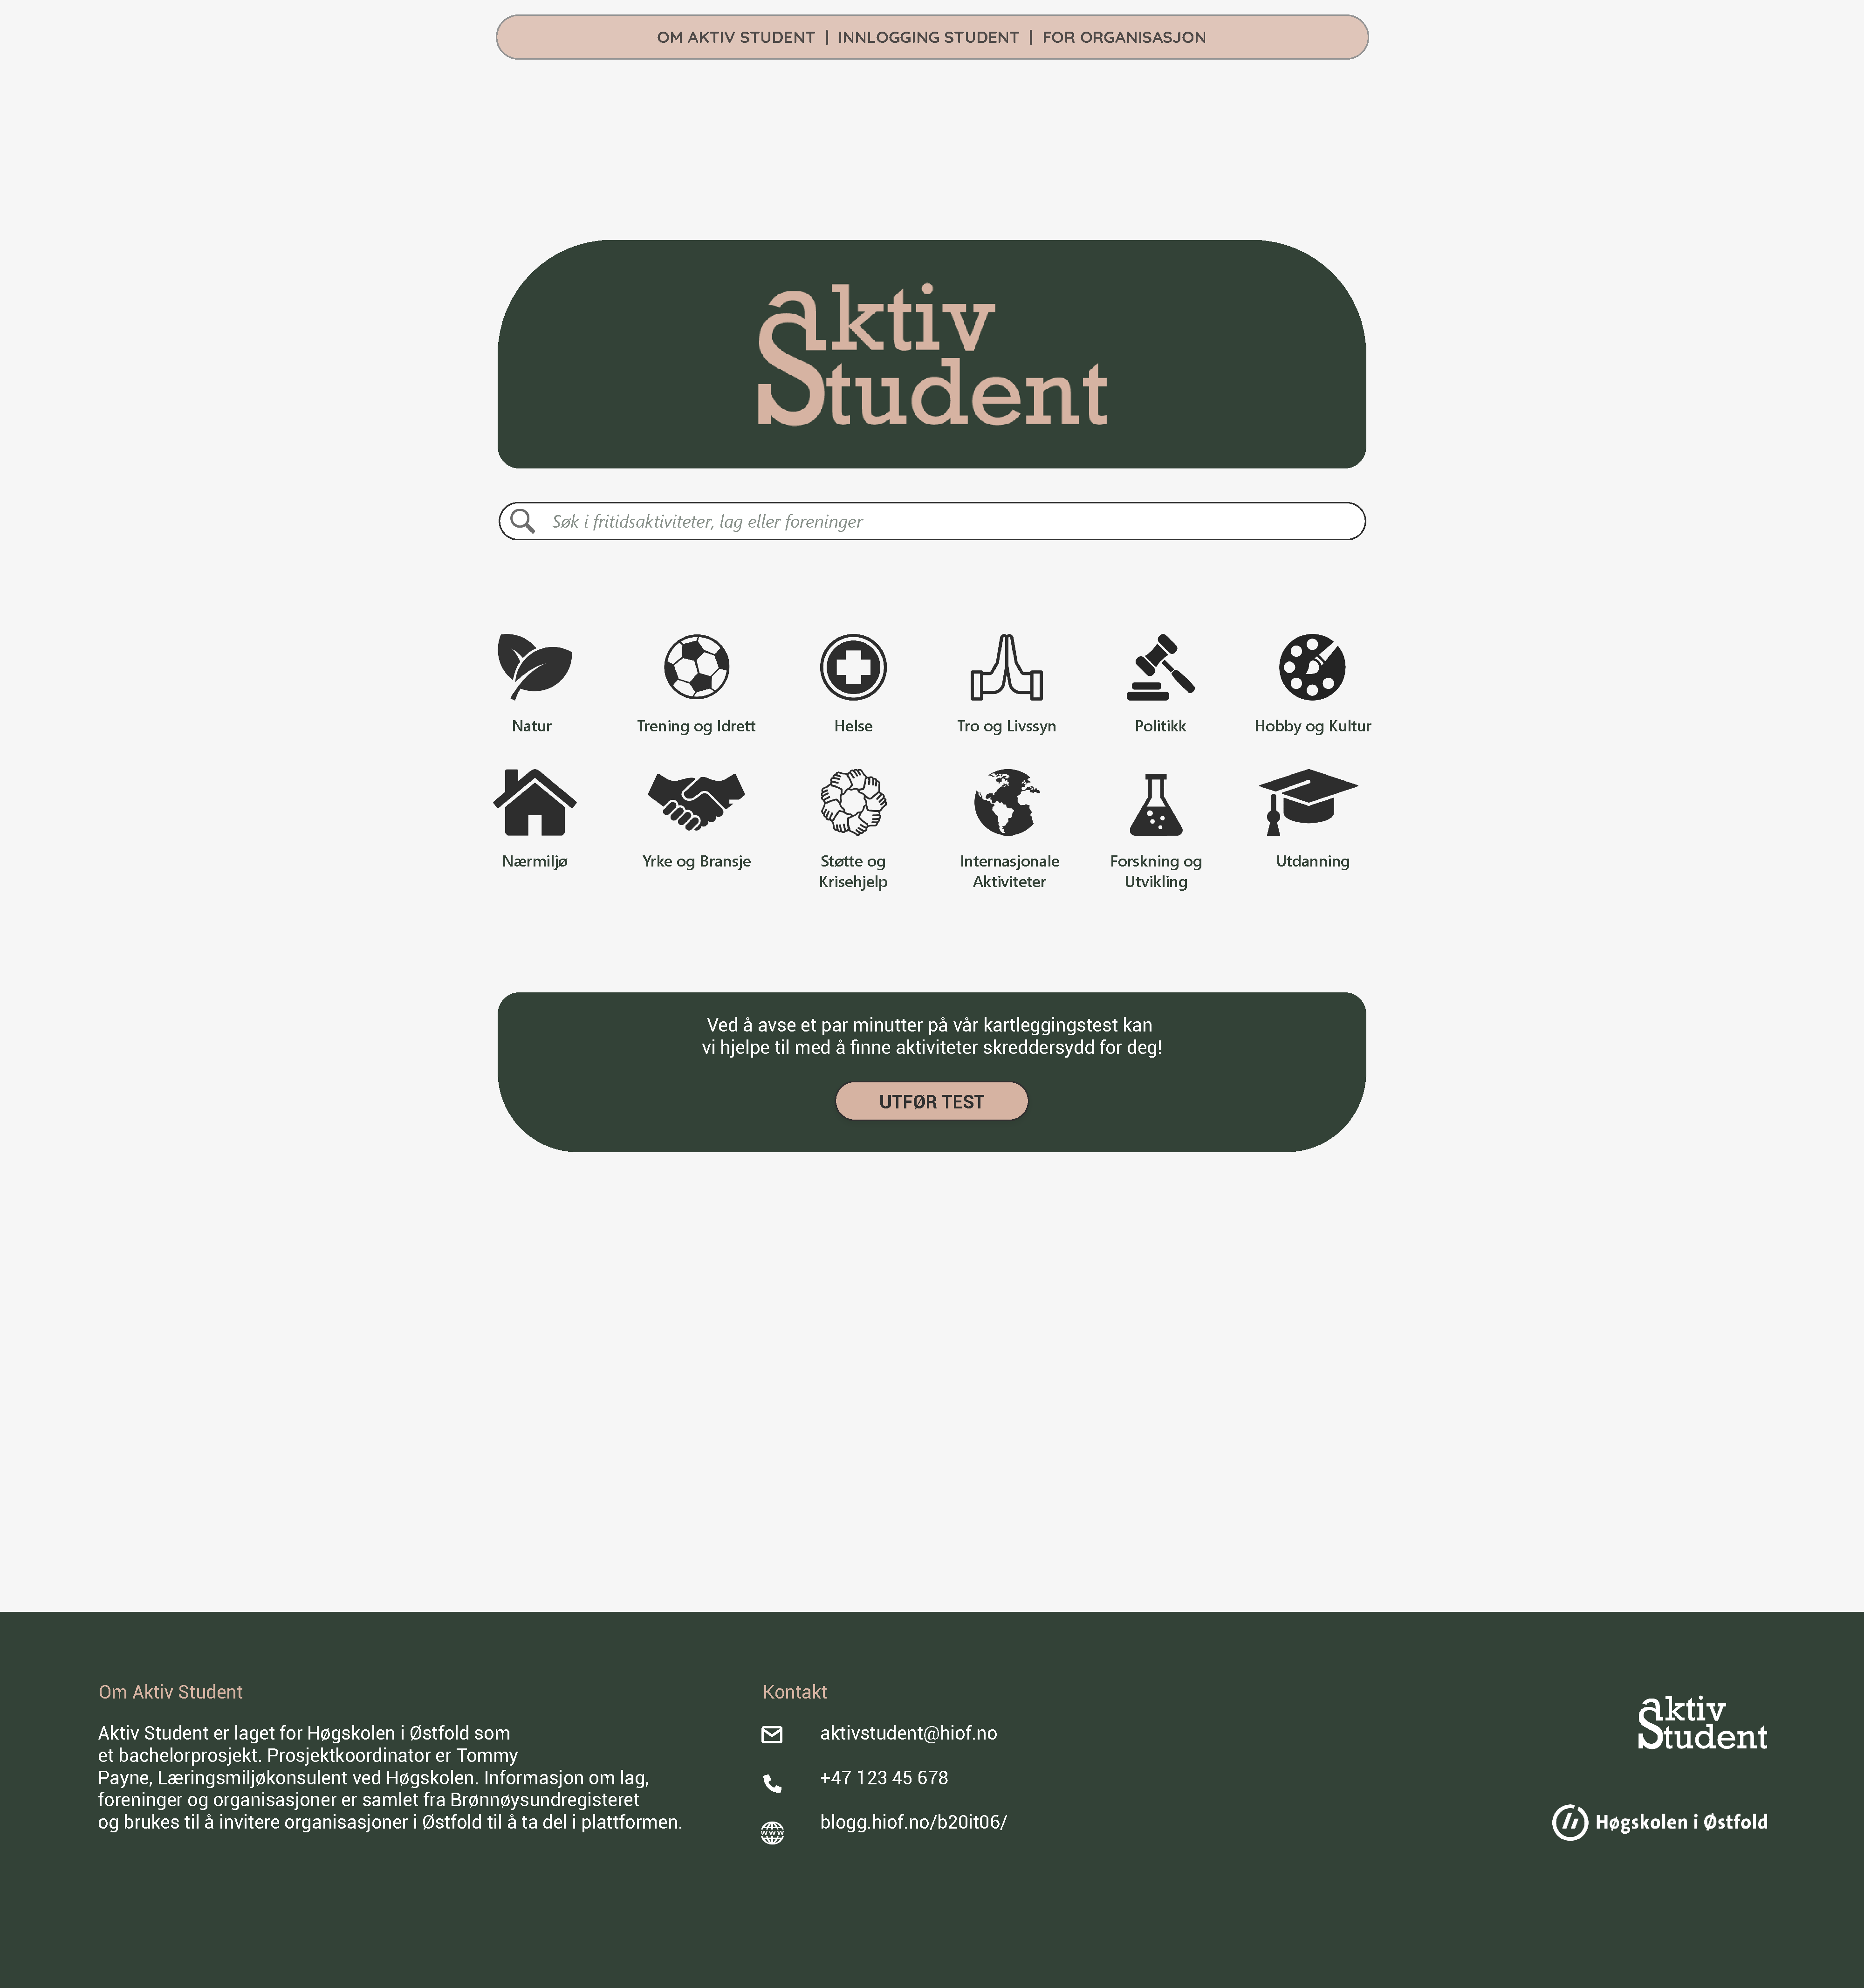
\includegraphics[width=.7\textwidth]{Illustrasjoner/Skisser-pdf/3.0/3-1-forside.pdf}
\caption{Adobe XD-skisse av plattformens forside}
\label{fig:3-1-forside}
\end{figure}

\paragraph{Layout og visuell design}
Valg innen plasseringen av elementer og design ble også gjort med tanke på minimalisme. Prosjektgruppen jobbet for å oppnå et layout som ikke virket rotete eller overfylt, med tydelige seksjoner for forskjellige elementer og en logisk plassering av elementer. Det ble eksperimentert med forskjellige mengder rom mellom elementene. I skisser med mye innhold var det viktig å ha nok mellomrom for å unngå at innholdet så tettpakket og rotete ut, men fortsatt ikke så mye mellomrom at brukeren kunne måtte scrolle langt ned for å finne innholdet den lette etter. Det ble også satt en standard for bredden på sidemargen, altså avstanden mellom innholdet og kanten av skissen. Denne bredden ble brukt på alle skissene som en kontinuitet og gjenkjennelighet i tjenesten, unntatt administratorpanel som var en selvstendig funksjon.

\paragraph{Ryddig visning av resultater}
Den endelige skissen av siden for søkeresultater vises i figur~\ref{fig:3-3-resultater-filtrering}. Å bruke utbrettsmeny var en naturlig løsning for denne tjenesten siden utbrettsmenyer allerede ble brukt både på forsiden og i kartleggingstesten, disse tiltakene bidro derfor til å skape et konsistent design.  


\begin{figure}[H]
\centering
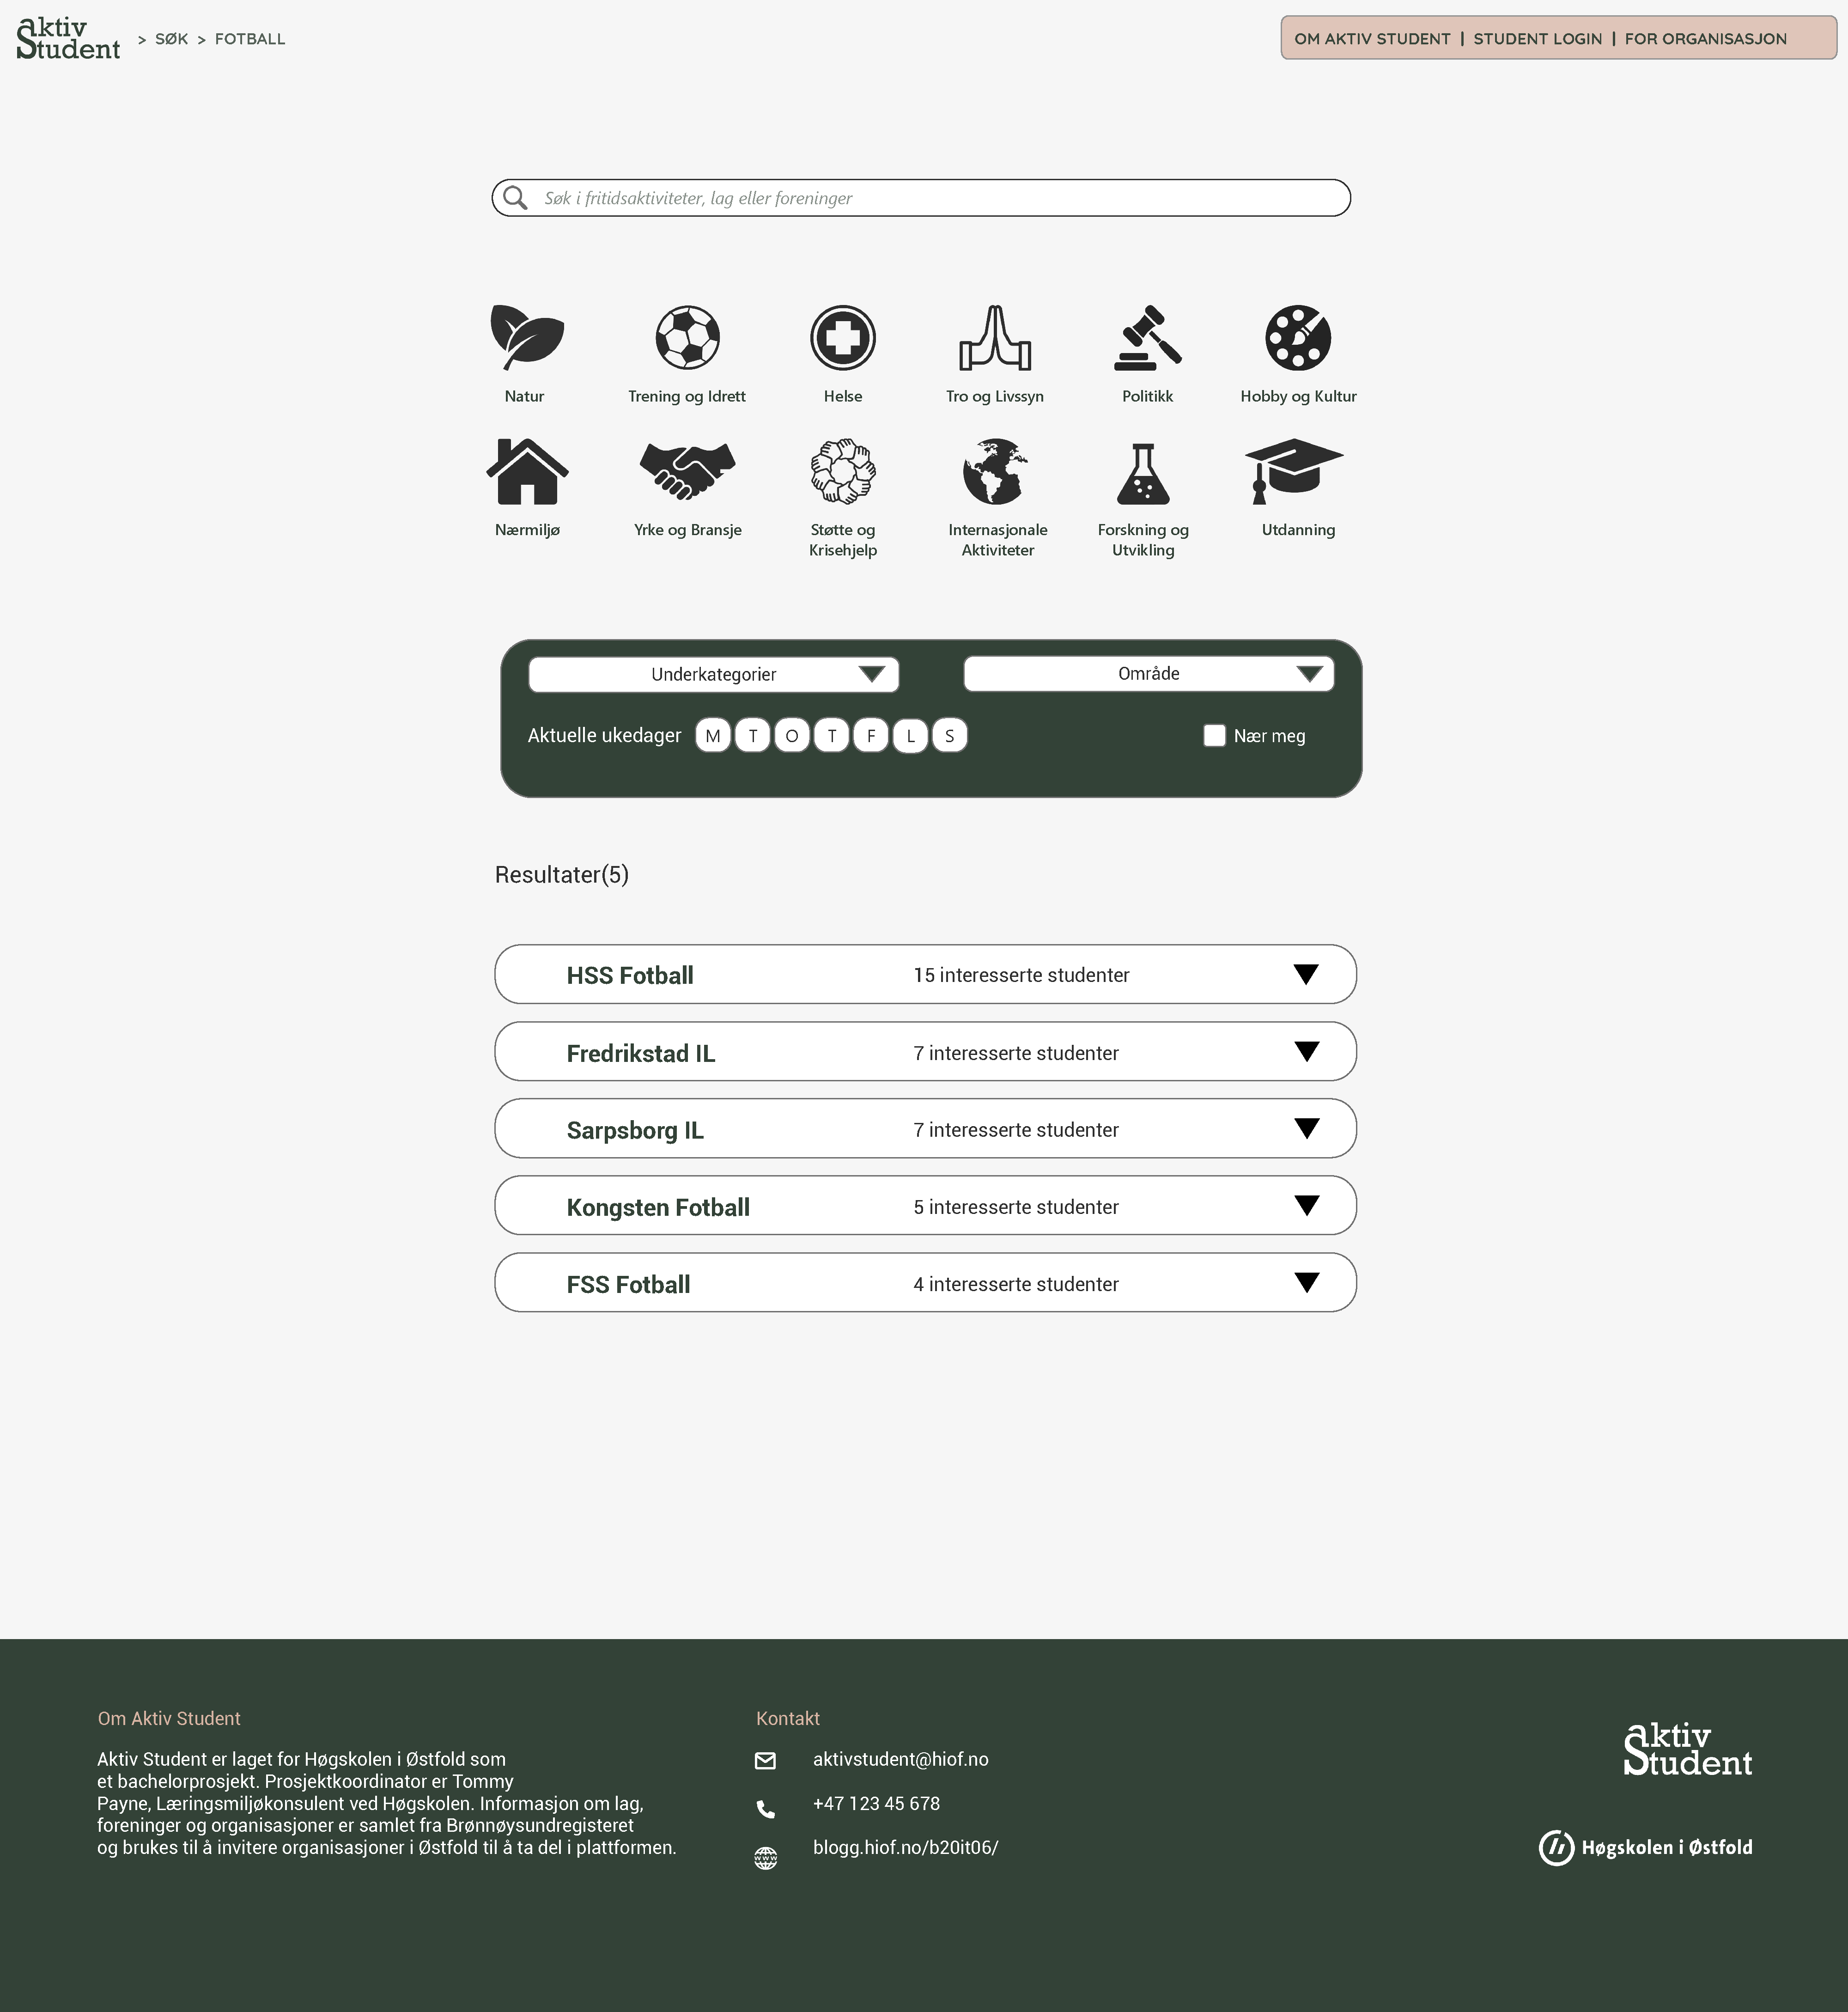
\includegraphics[width=.7\textwidth]{Illustrasjoner/Skisser-pdf/3.0/3-3-resultater-fotball.pdf}
\caption{Adobe XD-skisse av søkeresultatene etter bruker har trykket på underkategorien {\em Fotball}}
\label{fig:3-3-resultater-filtrering}
\end{figure}

\newpage
\subsection{Navigasjon}

Fundamentet til nettsiden Aktiv Student er bygget opp rundt databasen til Brønnøysundregisteret sin oversikt over fritidsorganisasjoner i Norge. Det kan dermed føre til en rekke utfordringer å presentere alt av nødvendig informasjon, noe som igjen kan medføre en risiko for å gi besøkende for mye innhold å se på til enhver tid.
\vspace{5mm}
Mennesker har kort oppmerksomhetsspenn, og forskning viser at en ordinær besøkende på en nettside bruker vel under ett minutt for å avgjøre om de blir værende eller ei\footnote{https://www.nngroup.com/articles/how-long-do-users-stay-on-web-pages/}. I et forsøk på å gjøre tjenesten uformell og spennende, skisserte vi en forside som inneholder et blikkfang i form av ikoner av kategoriene. Ved videre iterasjoner av skissene vedvarte ikonsettet etter positive tilbakemeldinger fra brukerundersøkelsene som ble gjort.

\begin{figure}[H]
\centering
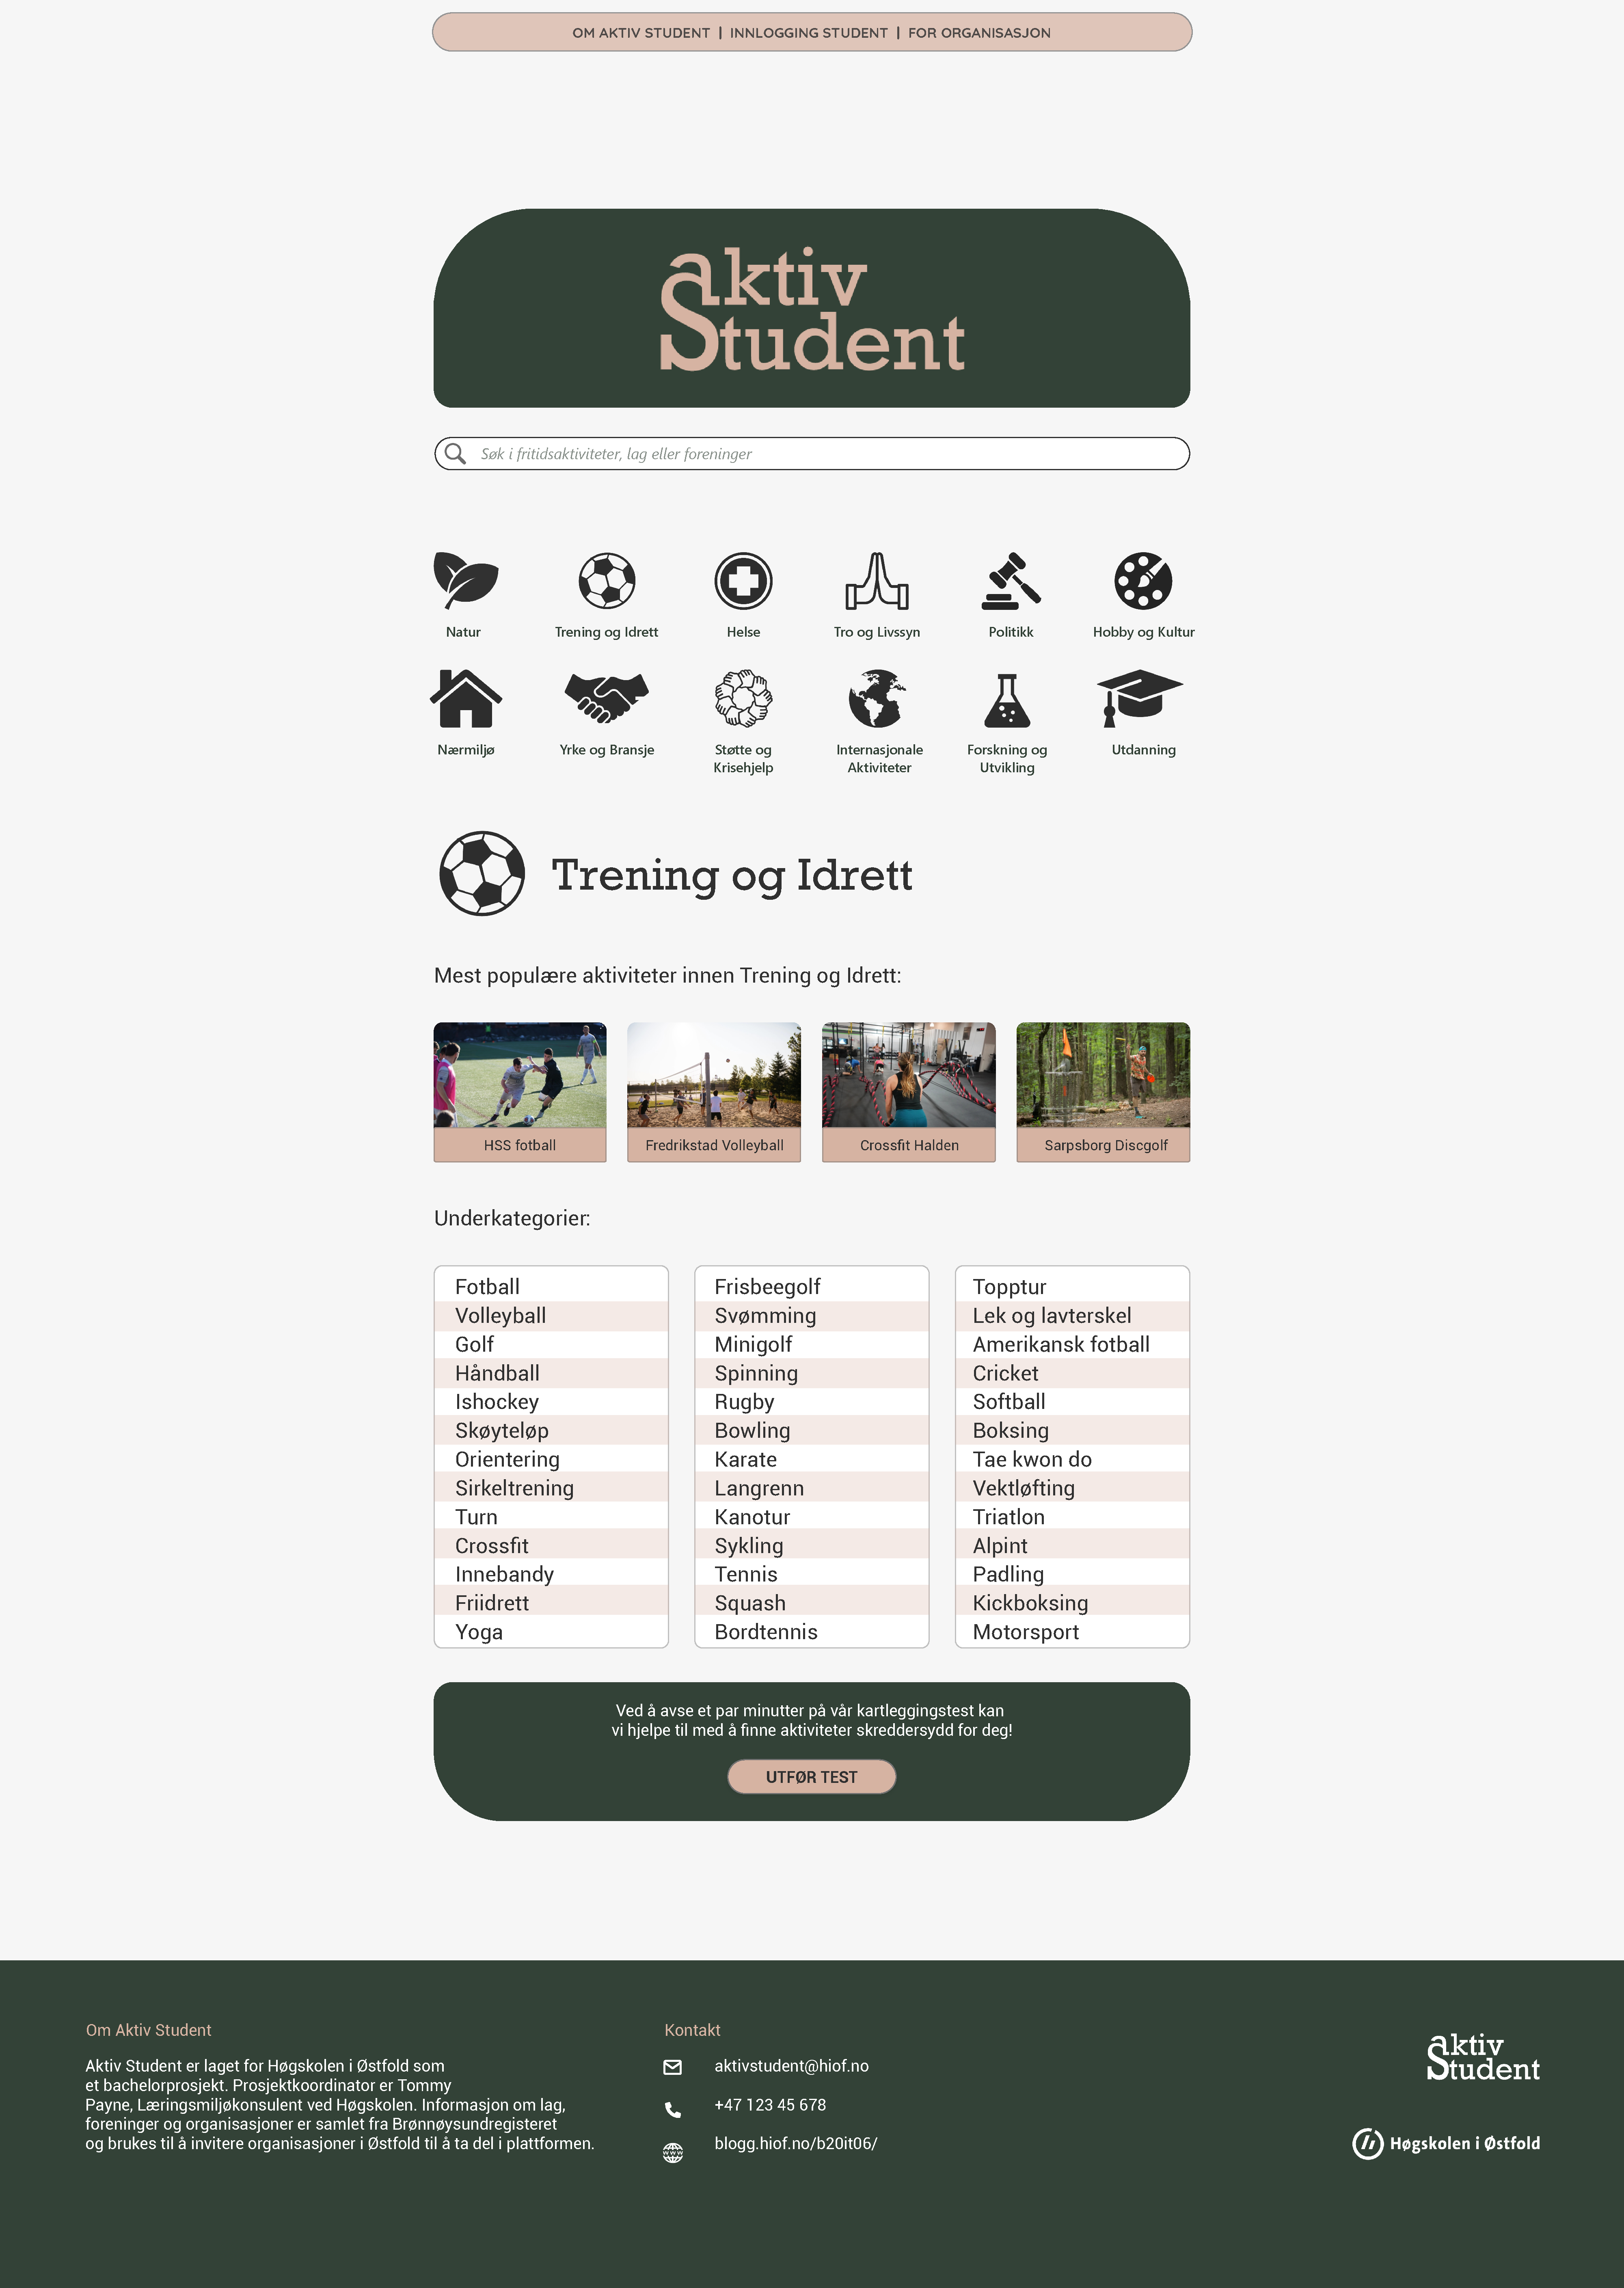
\includegraphics[width=.7\textwidth]{Illustrasjoner/Skisser-pdf/3.0/3-2-forside-trykket-kategori.pdf}
\caption{Adobe XD-skisse av plattformens forside etter bruker har trykket på kategori-ikonet for {\em Trening og Idrett}}
\label{fig:3-2-forside-utbrett}
\end{figure}


Ved klikk på et av ikonene (I figur 3.3 er Trening og Idrett brukt som eksempel) vil bruker få presentert en utbrettsmeny (uten å forlate forside) med oversikt over de mest populære lokale lag/foreninger i nærområdet, inklusive bilder for økt blikkfang, samt en liste med underkategorier av Trening og Idrett. Videre klikk på ett av de lokale lag/foreningene vil ta besøkende direkte til den foreningens organisasjonsside. Da har besøkende kun brukt to klikk for å komme til en aktuell organisasjonsside, inklusive prosessen i å først velge hvilken kategori de ønsker.

Ved fortsatt aktiv utbrettsmeny kan besøkende alternativt klikke på en underkategori som vil ta dem til en ny side. Søkeresultater og filtrering (vedlegg ~\ref{vedlegg:3-3-resultater-filtrering}). Der vil de mest populære lag og foreningene ligge ramset opp etter hva besøkende trykket på av underkategorier. Der finnes mulighet for å filtrere søket grundigere ved område, aktuelle ukedager som måtte passe for vedkommende, eller nytt valg av underkategori.

Disse to veiene inn til organisasjonssidene er selvsagt i tillegg til fritekstsøket på forsiden. Ett søk derifra vil ta besøkende direkte til Søkeresultater og filtrering, med søkeresultatene ramset opp under filtreringsboksen.

\begin{figure}[H]
\centering
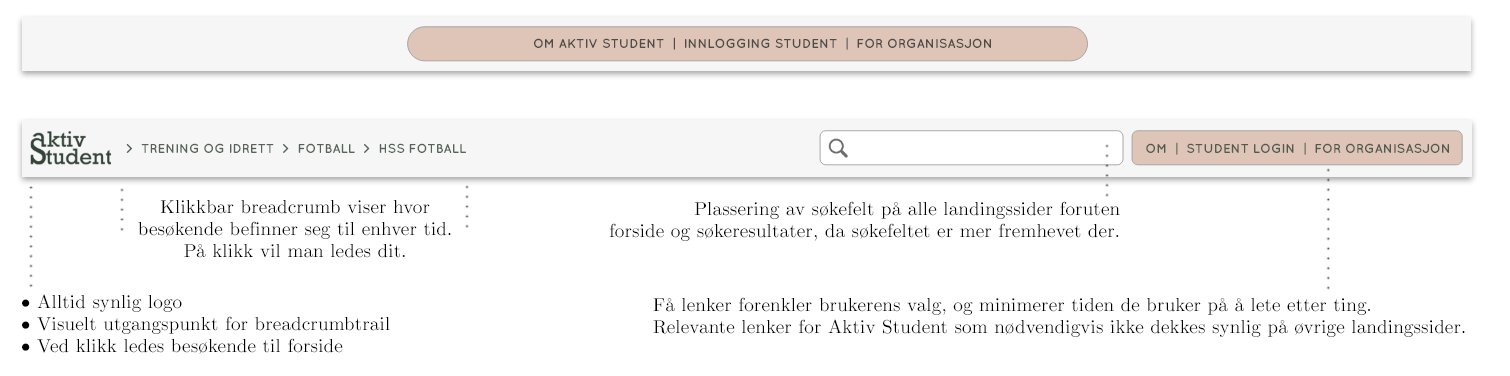
\includegraphics[width=1\textwidth]{Illustrasjoner/nav.png}
\caption{Øverst ligger nav-baren slik den ser ut på {\em forside} og {\em søkeresultater}. Under ser man nav-baren slik den ser ut på øvrige landingssider.}
\end{figure}

\paragraph{Bruk av tomrom (empty space)}

Prosjektet Aktiv Student har alltid indikert at det vil være aktuelt å presentere mye informasjon til brukere under sitt besøk. For å motkjempe at brukere skal behøve å føle at de drukner i all informasjon har prosjektgruppen gjort noen valg som omhandler lettleselighet. Innholdet som vises vil alltid bli vist i form av én kolonne eller «søyle» sentrert på skjermen, med 25\% tomrom ut ifra venstre og høyre kant.
Målet med dette er å kreve oppmerksomheten til brukeren, noe som reflekteres positivt fra brukerundersøkelser som er blitt gjort.

\vspace{5mm}

Unntakene som er blitt gjort fra denne regelen og hvorfor:\begin{itemize}
    \item Headernav
    \newline En naturlig plass å tillate grunnleggende informasjon å bruke hele skjermen horisontalt, siden den vil ligge direkte under adressenavigasjonen i de fleste nettlesere.
    \item Bilde for organisasjoner
    \newline En videreføring av headernav. Store, brede forsidebilder er et designvalg gjort for å stå i kontrast til brreg.no, som ikke tillater noen form for bildebruk.
    \item Kart og Footer
    \newline Plassert slik for å komplementere designvalgene gjort av Headernav og bilde for organisasjoner, og dermed avslutte siden.
\end{itemize}




\subsection{Tilrettelegging for brukergenerert innhold}
% Dette står det mye om i bøker om brukerorientert design, finn kilder. %
Det viktigste innholdet i tjenesten Aktiv Student vil være det som genereres av brukere, først og fremst innholdet som informerer om organisasjoner. Organisasjonsinformasjon ble derfor lagt stor vekt på i prototypen.

Et mål med informasjonssiden var at interesserte brukere kunne bli kjent med organisasjonen for å enklere kunne etablere et tillitsforhold, som nevnt av Anders Midtsundstad i prosjektgruppens intervju med han, oppsummert i delkapittel~\ref{section:init-brukerintervjuer}. Et annet mål var å legge til rette for at studenter kunne få all den informasjonen de trengte for å kunne delta, slik at mangel på informasjon ikke ble en hindring. Ettersom selve innholdet på en organisasjonsside produseres av en kontaktperson kunne ikke dette innholdet fastsettes i designet på forhånd, det som derimot kunne fastsettes var typen informasjon som kunne legges til.  I den endelige skissen av organisasjonssiden, vist i figur~\ref{fig:3-6-org-trykket-interessert}, inkluderes informasjon om hvem organisasjonen er, hva de gjør, hvordan man kan kontakte dem i tillegg til hvor og når man kan delta.

\begin{figure}[H]
\centering
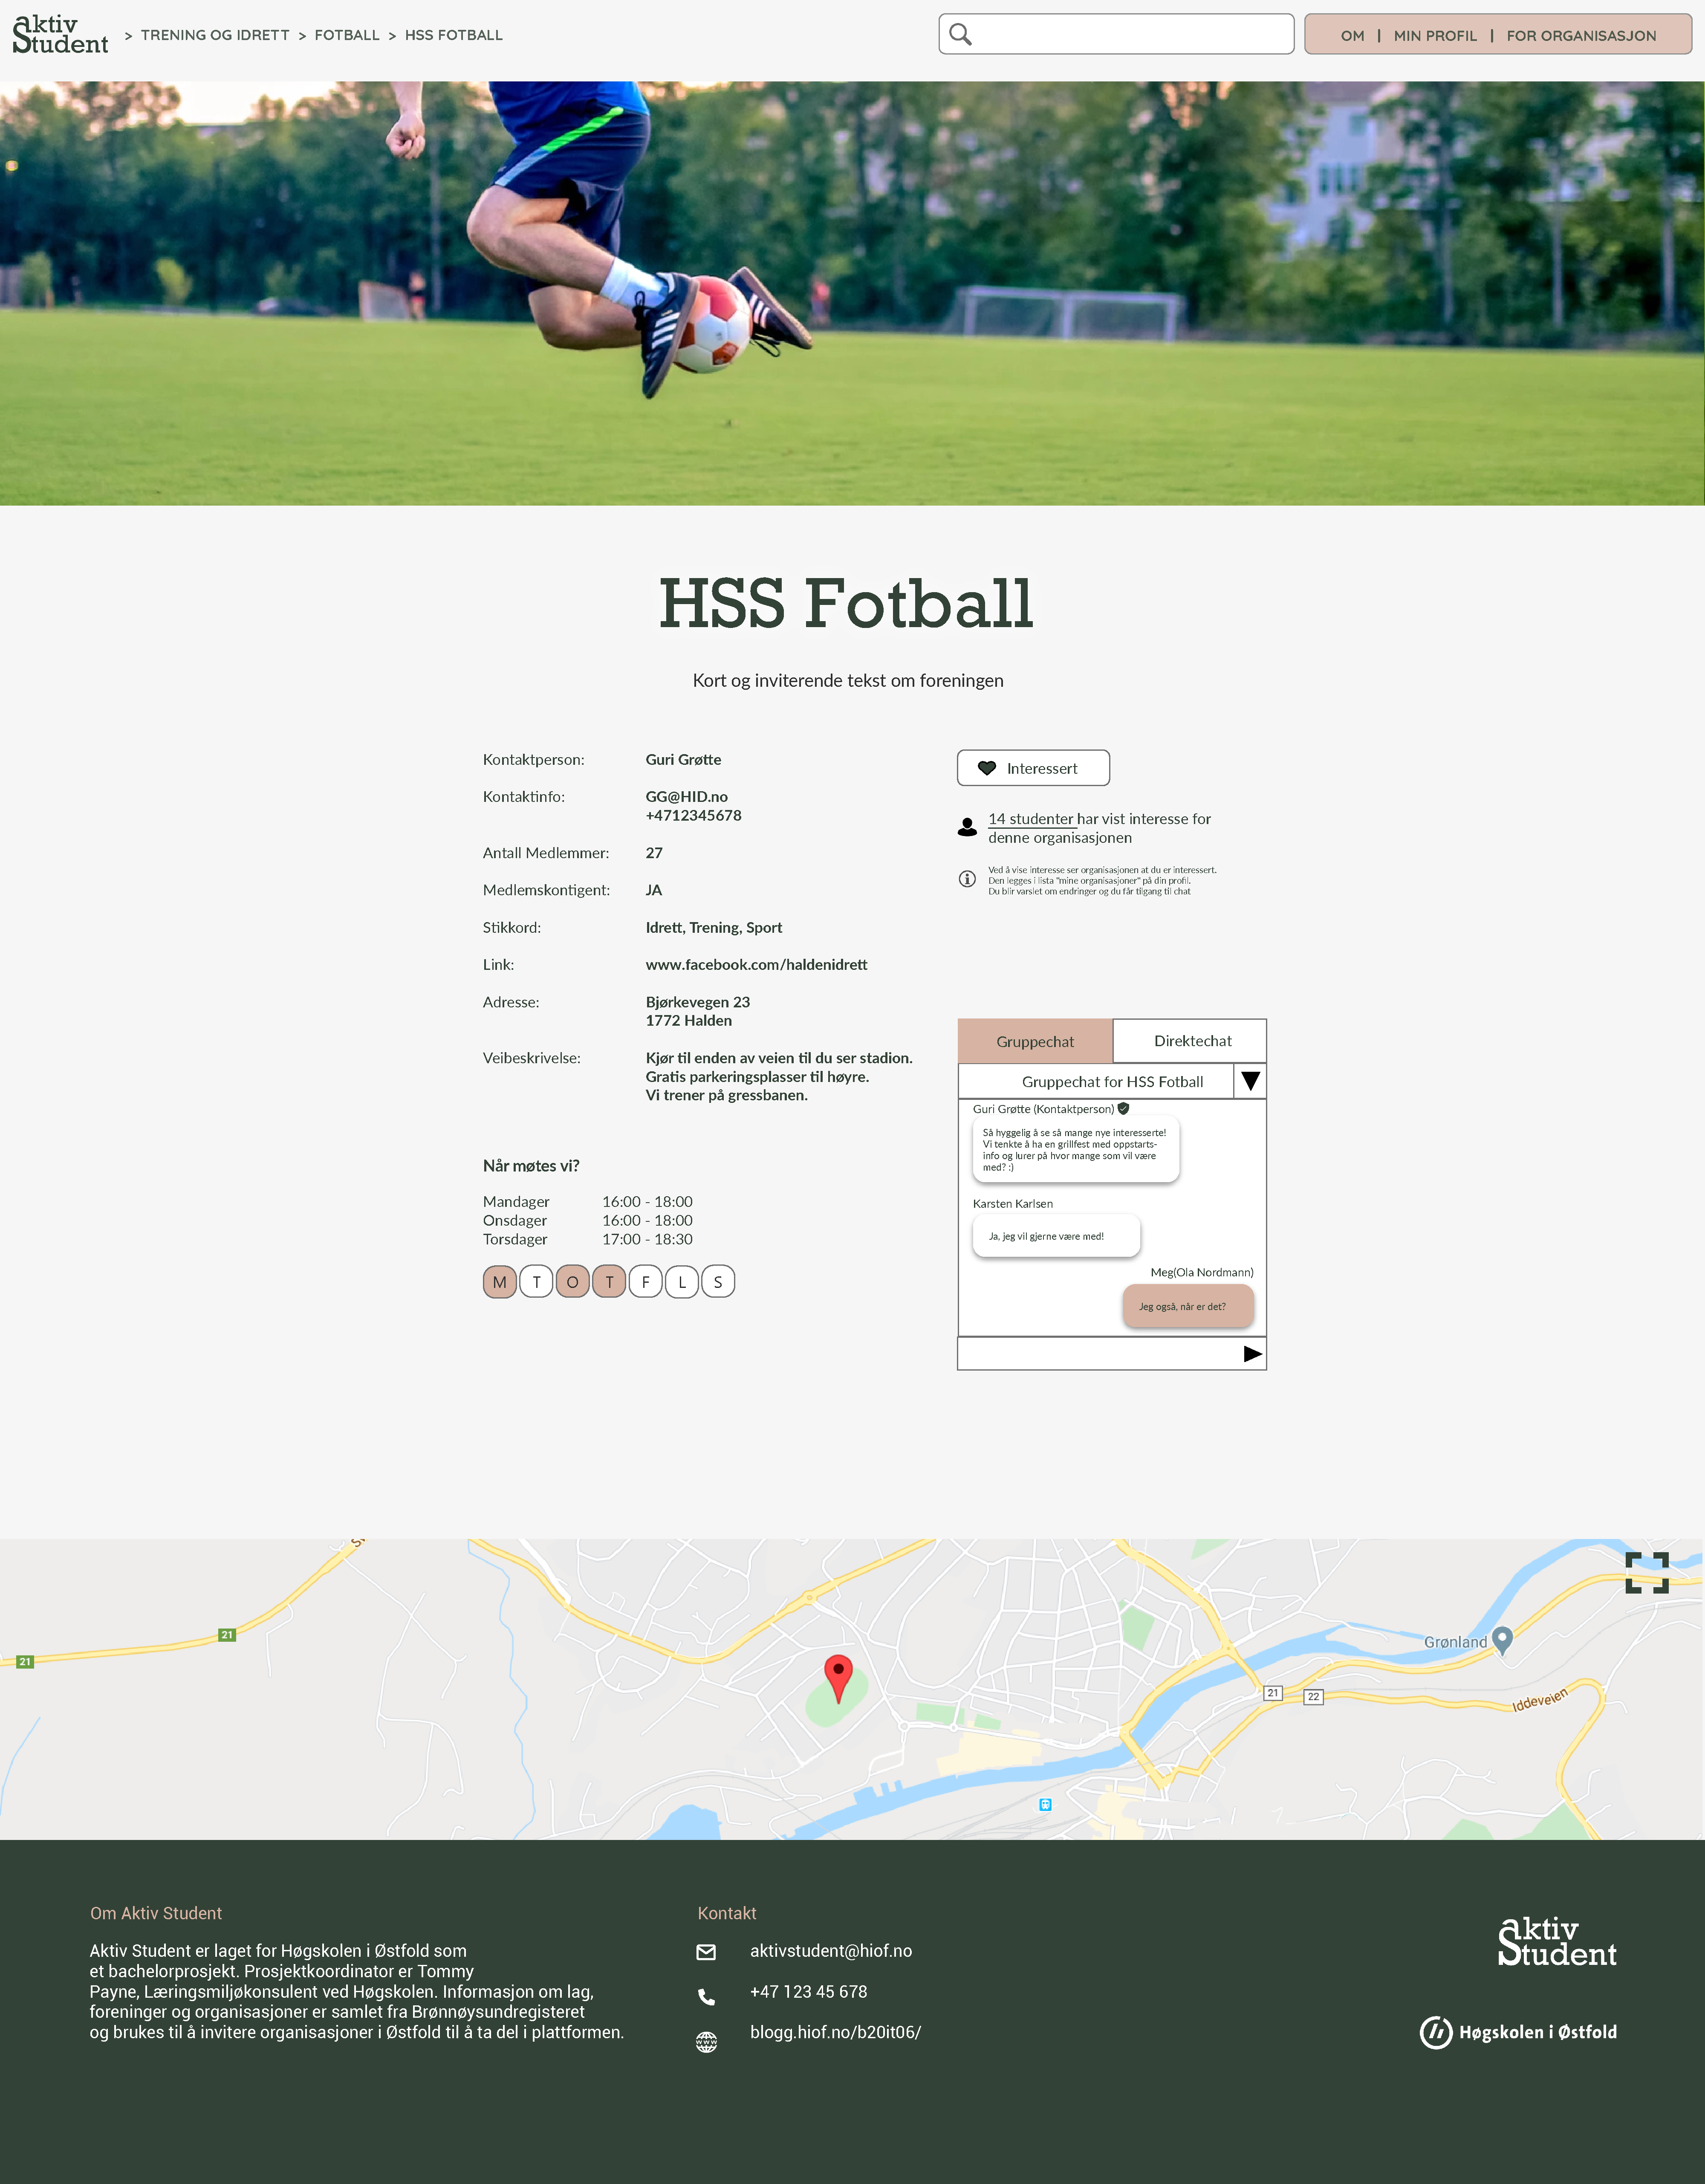
\includegraphics[width=.7\textwidth]{Illustrasjoner/Skisser-pdf/3.0/3-6-organisasjonsside-trykket-interessert.pdf}
\caption{Adobe XD-skisse av siden til eksempelorganisasjonen HSS Fotball etter bruker har trykket på {\em interessert}-knappen og får tilgang til chattefunksjonen}
\label{fig:3-6-org-trykket-interessert}
\end{figure}

Ettersom det kunne bli et problem at kontaktpersoner ikke la til utfyllende informasjon fordi de ikke hadde nødt ble det lagt inn oppfordringer til dette i designet. Dette gjøres gjennom en fremdriftslinje og enkel mulighet til å legge til og endre informasjon gjennom {\em endre}-knappen. Disse funksjonene vises på den innloggede organisasjonsprofilen, vist i figur~\ref{vedlegg:3-17-innlogget-org} i Tillegg~\ref{vedlegg:skisser3}. Tiltenkt funksjonalitet som ikke ble med i skissene er meldinger som minner kontaktpersonen om å legge til manglende informasjon, for eksempel i små dialogbokser på organisasjonens profil eller via varslinger i tjenesten eller på e-post.


\subsection{Spennende funksjonalitet}

\paragraph{Kartleggingstesten}
Testen inneholder et sett med ni eksempelspørmål med svaralternativene {\em ja}, {\em nei} og {\em nøytral}, der noen av disse spørsmålene hadde sett med mer detaljerte spørsmål som dukket opp i en utbrettsmeny om brukeren svarte {\em ja}. Den endelige skissen av kartleggingstesten vises i figur~\ref{fig:3-13-kartlegging-svart-ja}. Meningen er at alle spørsmål i testen knyttes opp til en eller flere aktivitetskategorier, dermed får hver kategori en poengsum etter hva brukeren har svart og aktuelle organisasjoner innen kategoriene med høyest poengsum presenteres for brukeren på resultatsiden. I prototypen er resultatsiden designet for at brukeren skal ha mulighet til å velge bort kategorier den ikke ønsker å ha med, vise kategoriene som interesser på sin profil og filtrere resultatene.

\begin{figure}[H]
\centering
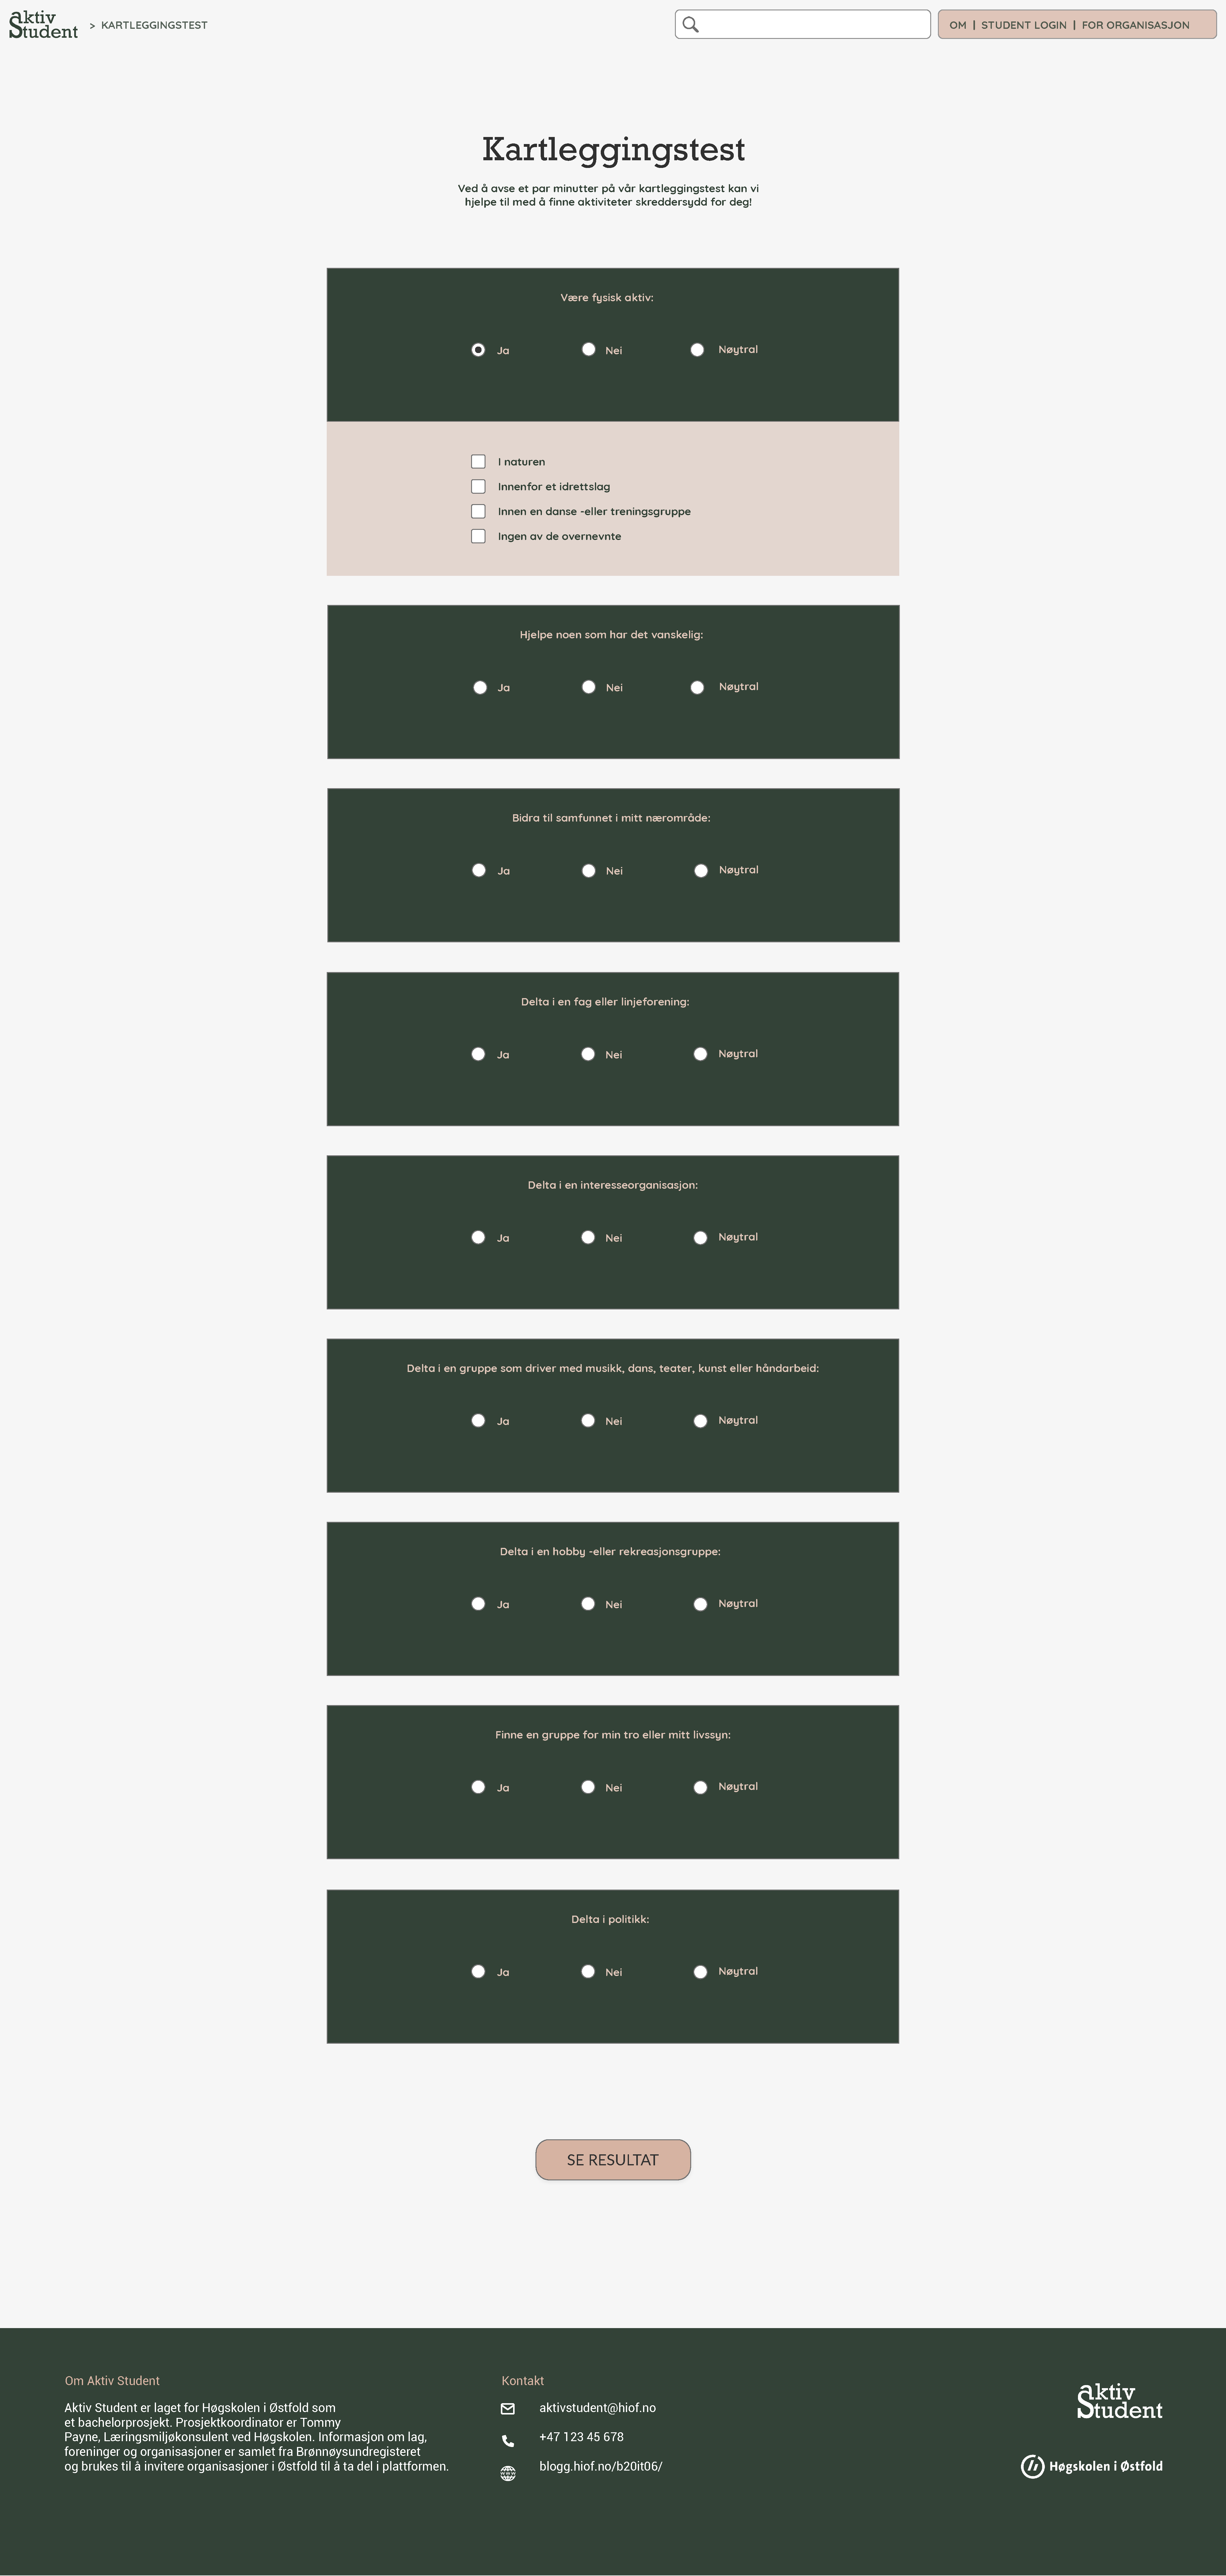
\includegraphics[width=.6\textwidth]{Illustrasjoner/Skisser-pdf/3.0/3-13-kartleggingstest-ved-svart-ja.pdf}
\caption{Adobe XD-skisse av kartleggingstesten med eksempelspørsmål etter bruker har svart {\em ja} på første spørsmål}
\label{fig:3-13-kartlegging-svart-ja}
\end{figure}

\paragraph{Chat-funksjonen}
Chat-funksjonen i prototypen viser muligheten til å delta i en gruppesamtale med alle som har trykket {\em interessert} på en organisasjon, i tillegg til å kunne snakke med kontaktperson direkte. Dette skaper en mulighet for å kunne snakke med en gruppe kun basert på felles interesse, der poenget ikke er hvem de er, men hva de har til felles. Funksjonen vises på skissen av en organisasjonsside i figur~\ref{fig:3-6-org-trykket-interessert}.

\paragraph{Mindre funksjoner og designvalg}
Prototypen ble utformet med tanken om å skape et spennende, lekent og uformelt uttrykk. Funksjonalitet og design som er implementert for å bidra til dette er: visning av mest populære aktiviteter, fremdriftslinje for å vise bruker hvor mange prosent den er fra å fullføre profilen sin, mulighet til å legge til organisasjoner i en liste med favoritter og få varsler fra disse og bruk av bilder som blikkfang. Alle disse forslagene, i tillegg til noen av prosjektgruppens egne idéer, ble brukt som virkemidler for å oppnå det ønskede uttrykket i tjenesten.

\subsection{Funksjoner og innhold i endelig prototype}


\begin{center}
\begin{longtabu}{|X|X|}
\caption{Liste over funksjoner i den endelige prototypen og hensikten med disse} \label{tab:funksjoner-ferdig-prototype} \\

\hline \multicolumn{1}{|c|}{\textbf{Funksjon}} & \multicolumn{1}{c|}{\textbf{Hensikt}} \\ \hline 
\endfirsthead

\multicolumn{2}{c}%
{{\bfseries \tablename\ \thetable{} -- fortsettelse}} \\
\hline \multicolumn{1}{|c|}{\textbf{Funksjon}} & \multicolumn{1}{c|}{\textbf{Hensikt}} \\ \hline 
\endhead

\endlastfoot

Innhenting av informasjon om organisasjoner fra Brønnøysundregistrene 
& Tjenestens datakilde, om en organisasjon enda ikke har opprettet profil vil det kun vises informasjon fra Brønnøysundregistrene på profilen med informasjon til studenter om dette \\ \hline

Oppfordring av organisasjoner til å opprette profil og legge inn mer info 
& Gir brukeren utfyllende og nyttig informasjon om organisasjonen \\ \hline

Brukere kan redigere brukerprofil 
& Gir bruker mulighet til å legge inn informasjon om seg selv enn det som hentes ut gjennom Feide-innlogging \\ \hline

Kartleggingstest med
\begin{compactitem}
    \item Oversikt over relevante organisasjoner
    \item Mulighet for kontakt med organisasjoner
    \item Mulighet for å se mer info om organisasjoner
\end{compactitem}
& Gjøre det enkelt og spennende for brukeren å oppdage nye organisasjoner \\ \hline

Bruker kan enkelt ta kontakt med organisasjoner
\begin{compactitem}
    \item {\em Interessert}-knappen
    \item Tilgjengelig kontaktinfo
    \item Oppfordre organisasjon til å legge til flere måter å ta kontakt på og være tilgjengelig
    \item Chat-funksjon
\end{compactitem}
& Øke sjansen for at en bruker kontakter en organisasjon og deltar på aktiviteter \\ \hline

God informasjon om aktiviteter 
\begin{compactitem}
    \item Informasjon om møtetider
    \item Bilde
    \item Har medlemskontingent/har ikke medlemskontingent
    \item Inkluderende ordbruk
    \item Oversiktlig
    \item Plassering og kart
    \item Antall medlemmer
    \item Antall interesserte studenter
    \item Link til nettside/sosiale medier
\end{compactitem}
&  Gi brukeren nok informasjon til at den føler seg trygg på å ta kontakt med organisasjonen og/eller delta\\ \hline

{\em Interessert}-knappen
& Lagre organisasjoner på sin profil, få varsler fra dem, få tilgang til chat \\ \hline


Fritekstsøk
& Gi brukeren mulighet til å utføre et målrettet søk på spesifikke aktiviteter \\ \hline

Filtrering på
\begin{compactitem}
    \item Område
    \item Kategori
    \item Møtedager
\end{compactitem}
& Gi brukeren mulighet til å utføre et målrettet søk etter kriterier som kan være viktig for den \\ \hline

Velge kategori og se aktiviteter
& Brukere som vet hvilke type aktiviteter de er interessert i kan oppdage hvilke tilbud som fins innen disse kategoriene \\ \hline

Mest populære aktiviteter  
& Presentere brukere med et tilbud uten at de trenger å gjøre noe, gi brukeren et tilbud der de vet det er mange deltakere \\ \hline

Chat-funksjon  
\begin{compactitem}
    \item Gruppechat
    \item Direktechat
\end{compactitem}
& Gi brukere en måte og kontakte kontaktperson for organisasjonen på og kommunisere i et sosialt felleskap med andre interesserte studenter \\ \hline

Innlogging
\begin{compactitem}
    \item Feide-innlogging
    \item Tradisjonell innlogging
\end{compactitem}
& Innlogging for studenter ved hjelp av Feide eller tradisjonell innlogging og tradisjonell innlogging for organisasjoner. Feide henter ut navn, e-post og studieprogram for studenter og viser dette på profilen deres \\ \hline

Registrering 
& Enkel opprettelse av profil for bruker og organisasjon. Studenter som logger inn med Feide kan hoppe over dette \\ \hline

Om oss 
& Enkel og beskrivende side som forklarer hva Aktiv-Student tjenesten er  \\ \hline

Organisasjonsprofil 
\begin{compactitem}
    \item Endre informasjon
    \item Fremdriftslinje for ferdigstilling av profil
    \item Snakke med interesserte studenter i chat
\end{compactitem}
& side for organisasjoner hvor de kan legge til informasjon og innhold om seg selv, endre informasjonen sin og snakke med interesserte studenter i direktechat eller gruppechat  \\ \hline

Administratorpanel 
& Side hvor admin kan gjøre endringer, invitere organisasjoner, godkjenne endringer gjort av organisasjoner, håndtere rapporteringer fra brukere og se statistikk for tjenesten \\ \hline



\end{longtabu}
\end{center}

\subsection{Resultat i forhold til brukerens kravspesifikasjon}

\subsubsection{Tjenestens innhold}

\fet{Det skal være enkelt å finne oversikt over tilgjengelige aktiviteter}

Antall hovedkategorier har blitt kortet ned fra de 14 funnet på brreg.no ned til 12. Disse 12 har blitt testet for forståelse og synlighet, og implementert deretter. Kategoriene presenteres som symboler som vises prominent frem på forsiden til Aktiv Student. Klikk på de viser underkategorier til valgt kategori samt de mest populære lokale organisasjonene som driver med det. To klikk fra forsiden vil derfor fremvise nytteverdig informasjon for besøkende. 

En kartleggingstest er også utviklet for å kategorisere brukeren selv sine behov og ønsker, ved tilfelle at de trenger en pekepinn for å finne aktuelle aktiviteter.

\fet{Det skal være enkelt å søke på og finne frem til en spesifikk aktivitet}

Et søkefelt vil ligge synlig og dominerende på forside. Herfra kan man søke på alt fra kategorier til navn på foreninger, lag og organisasjoner. Dette dominerende søkefeltet vil også finnes på "Søkeresultater og filtrering", en dedikert landingsside for å filtrere søk etter underkategorier, område og aktuelle ukedager. Foruten disse vil søkefeltet finnes på toppen av hver side i navigasjonsmenyen.

\fet{Systemet skal hjelpe brukeren å finne potensielle aktiviteter som passer for den}

En kartleggingstest er utviklet og tilgjengelig fra forsiden på tjenesten. Ved å oppfordre bruker til å bruke få minutter på denne, kan bruker få fremlagt en rekke aktiviteter som kan være aktuelle og interessante.

På de øvrige organisasjonssidene kan man se hvor mange andre studenter som er interessert, og man kan kan klikke på de forskjellige for å se hva de igjen er interessert i av organisasjoner. Formålet med dette er å indirekte fremlegge for brukere hva annet av aktiviteter de kan vise interesse for.

\fet{Informasjonen skal være oppdatert og korrekt} og \fet{Det skal være relevant og utfyllende informasjon om aktivitetene}
Brukerprofilene til organisasjoner består av en viss mengde ferdigutfylt info som blir hentet fra brreg.no sin database. I tillegg oppfordres organisasjoner til å føre inn informasjon som er både inviterende og relevant for studenter. Kontaktpersoner, kontaktinfo, webadresser og møtetider er noen av de mest aktuelle.

Oppfordringen for å føre inn slik informasjon vises iform av en fremdriftslinje (progress bar) på profilen til organisasjonen. Dette er ment som et insentiv for å engasjere organisasjonene til å skrive.

\fet{Det skal være enkelt å komme i kontakt med andre brukere og organisasjoner}
Aktiv Student kan senke terskelen for kontakt mellom studenter og organisasjoner ved å introdusere en chat-funksjon. Denne funksjonen er tilgjengelig for innloggede brukere, og fungerer slik at bruker melder interesse for en organisasjon, for så å få tilgang til chatten. Her kan alle som også har vist interesse for organisasjonen delta, og organisasjonens kontaktperson oppfordres til å være delaktiv.

Her vil det være uforpliktende å snakke sammen. Brukere kan svare når de vil eller har mulighet. Stresset som noen kan føle på ved å ringe foreninger eller ukjente mennesker vil forsvinne.

\fet{Det skal være lav terskel for å ta kontakt med andre brukere og organisasjoner}
Tjenesten Aktiv Student benytter seg ikke av venneforespørsler. Det er meningen at man heller kan prate med likesinnede i chatten til de respektive organisasjonene. Dette kan medføre til gode samtaler og økt kontakt blant de som ønsker det. Det oppfordres til at organisasjonene selv tar den første kontakten i chatten.

\fet{Systemet skal fasilitere for at brukere kan delta på aktiviteter sammen}
Tjenesten legger til rette for at brukere med felles interesser kan prate sammen. Medlemmer av organisasjonen kan for eksempel avtale aktiviteter og samkjøring sammen. Synlig navn og e-post vil gjøre kommunikasjon og planlegging enklere for deltakere.

\fet{Systemet skal være spennende og attraktivt å bruke}

Det er lagt vekt på at tjenesten og nettsiden den befinner seg på skal inneha en hyggelig og inviterende tone. Dette utføres ved hjelp av hyggelig ordlegging i tekst, duse farger, bruk av bilder og symboler.

Kartleggingstesten er en funksjon som kan engasjere besøkende til å utforske potensielle aktiviteter skreddersydd for dem.

En prat med likesinnede er målet bak en chat-funksjon som kun eksisterer inne på en organisasjon sin profilside.

\subsubsection{Teknisk funksjonalitet}
\fet{Det skal gå an å filtrere søk på relevante kriterier}
Det ble gjort en undersøkelse på lesbarhet og forståelighet rundt betegnelsene som finnes på brreg.no per i dag. De forbedrede termene vil bli brukt som valgmuligheter ved et søk og filtreringsside som tjenesten tilbyr.

\fet{Tjenesten skal være intuitiv og gjenkjennelig}
Tiltak: samme type design på flere sider, brukt forståelig språk og symboler, beskrivende tekster

Utseende på tjenesten vil forbli lik på alle landingssider, gjenkjennbare symboler vil pryde forside og kategorioverskrifter. Dette for å gjøre brukere visuelt kjent med tjenesten. Beskrivende tekster vil medføre til økt forståelse på hva tjenesten tilbyr.

\fet{Designet skal være minimalistisk}
Prototypen inneholder mye tomrom mellom elementer og ingen overflødige elementer på landingssidene. Velvalgte ord resulterer i kortfattede og informasjonsrike informasjontekster.

\fet{Det skal være enkelt å finne frem dit man skal i tjenesten}
Navigasjonen på prototypen er utviklet for besøkende å bruke minst mulig klikk for å komme dit de vil. Dette er forsterket fra forsiden og ut til de øvrige sidene. Det tar eksempelvis to klikk for bruker å finne en relevant aktivitet for dem fra forsiden.

\fet{Innholdet som vises skal være kun det nødvendige}
Tjenesten fremlegger informasjon ettersom hva bruker gjør i form av utbrettsmenyer ved klikk. Kun mest nødvendig informasjon vil vises til enhver tid.

\fet{Tjenesten skal ikke inneholde forstyrrende funksjoner eller designmomenter}
Avgjørelser ble tatt som omhandlet hvordan å integrere og plassere elementer og funksjoner der de føltes mest naturlig. Prosjektteamet skrapet ting som ikke fungerte, slik som eksempelvis hele konseptet rundt aktivitetsvenn.

\fet{Fargepaletten skal være enkel og minimal}
Det ble brukt noe tid på utforske fargebruk til prototypen. Vi endte opp med å bruke to duse nyanser av forholdsvis lys rosa og mørk grønn.

\fet{Menyen skal kun inneholde det nødvendige}
Øverst på siden finner man menyen. I venstre hjørne er ligger en hjem-knapp i form av Aktiv Student logo. Ut ifra logoen følger en klikkbar breadcrumb-sti som viser hvor besøkende befinner seg til enhver tid. Et søkefelt blir liggende til venstre for lenker til {\em Om oss, Student login} og {\em For Organisasjon}.

\fet{Søkefeltet skal være synlig og lett tilgjengelig}
På landingssidene {\em Forside} og {\em Søkeresultater} finner man søkefeltet fremtredende midt på siden. På de øvrige sidene vil den bli lagt til venstre for lenkene i navigeringsmenyen øverst på siden man er på.


\section{Resultater fra undersøkelse av hypoteser}
De fire hypotesene som prosjektgruppen utarbeidet i begynnelsen av prosjektet ble undersøkt gjennom gruppens egne brukerundersøkelser, konsultasjon av fagpersoner og relevant forskning og faglitteratur. Dette ble gjort parallelt med arbeidet med skissene nettopp fordi hypotesene oppsummerte antakelser og spørsmål som prosjektgruppen ønsket å få svar på underveis i prosessen for å kunne utarbeide en god prototype.

En sikker bekreftelse eller avkreftelse av hypotesene var enten ikke mulig eller ikke praktisk gjennomførbart for prosjektgruppen, men dette var heller ikke hensikten med hypotesene. Hypotesene ble brukt som en ledetråd for å finne de viktigste fokusområdene i videre undersøkelser og dermed i design av tjenesten. Det var derfor viktigst for prosjektgruppen å kunne bruke funn fra undersøkelsene i prosjektarbeidet og finne ut om funnene styrket eller svekket hypotesene, slik at fokusområdene eventuelt kunne justeres etter som.

\subsection{H1: En tjeneste som tilrettelegger for å delta sammen med andre likesinnede kan senke terskelen for å delta på en aktivitet}

\paragraph{Brukerintervjuer}
Hypotese 1 fikk støtte allerede under de initielle brukerintervjuene, beskrevet i delkapittel~\ref{section:init-brukerintervjuer}. 8/8 deltakere av brukerintervjuene svarte at å få med en venn eller bekjent ville gjort det enklere for dem å bli med på en organisert fritidsaktivitet. Dessuten svarte 7/8 deltakere at de tidligere hadde deltatt på en fritidsaktivitet fordi venner eller bekjente var med. De fleste av disse svarte også at det sosiale fellesskapet var en viktig grunn til at de valgte å delta. Noen svarte også at de ikke ville deltatt om de ikke hadde kjent til noen andre som deltok på aktiviteten.

\paragraph{Invitasjon til deltakelse gjennom mellomledd}
7/8 deltakere av de initielle brukerintervjuene svarte at gitt at de hadde en bekjent som var medlem i en organisasjon de var interesserte i, ville de tatt kontakt med den bekjente for å finne ut mer om organisasjonen. På den andre siden ville kun 2/8 deltakere tatt direkte kontakt med organisasjonen. Dette bygger opp under antakelsen om at personer i målgruppen heller ønsker å tilnærme seg organisasjonen gjennom et mellomledd enn å ta kontakt og delta alene. 

Dette ble gitt videre støtte av fagperson Anders Midtsundstad, som har utviklet metoden Fritid med Bistand \footnote{https://www.fritidmedbistand.no/}. Midtsundstad skrev i en samtale med prosjektgruppen via e-post at \say{I metoden Fritid med Bistand er det saksbehandler som har et ansvar i arbeidet med metoden til å legge til rette for deltakerne. Dette innebærer behov for å bruke den tid som kreves for å etablere tillit mellom metodens aktører. [...] I metoden Fritid med Bistand handler det om unge og eldre med ulike former for bistandsbehov. Studentene som er deres målgruppe har ofte en annen situasjon, men tillitsrelasjonen må en alltid forholde seg til. Det betyr i praksis at en tredjeperson bør invitere til fellesskapet} \cite{MIDTSUNDSTAD-EPOST:14}. 

Intervjuet med kvinnen som jobber i NAV indikerer mye av det samme. Kvinnen sa i intervjuet at \say{det kan virke som mange må ha noen som kan fysisk følge dem til arrangementer, ei hånd å holde i. Det hjelper ikke hvor mange tilbud man får når man er alene} \cite{NAV-INTERVJU:16}. Her var altså hjelp fra et mellomledd og deltakelse sammen med noen andre sentralt for at personene skulle tørre å dra på arrangementer. 

\paragraph{Konklusjon av undersøkelse av hypotese 1}
Etter undersøkelse av hypotese 1 kom prosjektgruppen frem til at ved å tilrettelegge i tjenesten for å delta sammen med andre eller å bli invitert til å delta av et mellomledd er det sannsynlig at dette kan føre til at studenter blir mer motivert til å delta. Gjennom at det sosiale og menneskelige aspektet ved tjenesten blir gjort tydelig kan studenten få større tillit til organisasjonen \cite{MIDTSUNDSTAD-EPOST:14}. Uten å utvikle tjenesten og teste denne i bruk er det dog umulig å si sikkert om tjenesten faktisk vil senke terskelen for å delta på aktiviteter, men prosjektgruppens funn styrker hypotese 1.

\subsection{H2: Studenter ved HIØ syns det er vanskelig å finne en oversikt over aktivitetstilbud}

\paragraph{Brukerintervjuer}
Svar fra de initielle brukerintervjuene støttet opp under hypotese 2. 6/8 deltakere svarte at å få bedre oversikt og tilgang til aktivitetstilbud ville gjøre det enklere for dem å delta på en aktivitet. Det som samtidig ble nevnt var vanskeligheten med å finne frem til kontaktinformasjon eller informasjon om hvordan man kunne delta på en aktivitet. 7/8 deltakere svarte at lett tilgjengelig kontaktinformasjon til organisasjoner spilte en viktig rolle i om de ville ta kontakt eller ikke. I tillegg svarte 8/8 deltakere at de ville tatt kontakt med en interessant organisasjon om det hadde eksistert gode tjenester som gjorde det enkelt å ta kontakt.

Deltakerne som ikke hadde deltatt på en organisert fritidsaktivitet i løpet av studietiden ble spurt om hva som holdt dem fra å delta. Én deltaker svarte \say{det er for dårlig tilbud. Jeg har sjekket tilbudet til HSS men ingenting der fenger.} En annen deltaker sa at han \say{vet ikke hva som er tilgjengelig og da gidder jeg ikke å begynne å lete.} Det ble også nevnt av flere deltakere at det var viktig for dem å ha lett tilgang til god og oppdatert informasjon om organisasjonene, ettersom flere av deltakerne heller ville lest om dem og møtt direkte opp på møte enn å tatt kontakt med organisasjonen først.

\paragraph{Mangler ved dagens aktivitetstilbud}
I alle rundene med brukerundersøkelser som ble gjennomført ble deltakerne spurt om sine tanker om konseptet Aktiv Student. Svarene som kom frem pekte på en mangel på et oversiktlig aktivitetstilbud for studenter ved HIØ i dag. I førsteinntykkstesten av skisser 1.0 sa en deltaker at han \say{liker konseptet, det er mangel på dette i dag og studenter ved høgskolen trenger det}. I brukertesten av skisser 2.0 ble en ny gruppe med deltakere spurt samme spørsmål. Det ble sagt av en deltaker at plattformen \say{svarer på et eksisterende behov ved høgskolen.} En annen deltaker sa at han ville brukt plattformen fordi \say{informasjon om organisasjoner på HIØ i dag er overfladisk og spredt overalt}.

Et viktig element i alle brukerundersøkelsene var at deltakerne skulle kunne snakke fritt og med så få føringer fra prosjektgruppen som mulig. Problemene med aktivitetstilbudet ble følgelig tatt opp på eget initiativ av studentene som deltok i undersøkelsene. Av mange deltakere ble denne problemstillingen også nevnt som første tema i samtalene om fritidsaktivitetstilbudet for studenter ved HIØ.

\paragraph{Konklusjon av undersøkelse av hypotese 2}
Etter å ha snakket med til sammen 13 forskjellige studenter ved HIØ, noen av dem i flere omganger, forelå det mange svar og bemerkninger som styrket antakelsen om at studenter syns at dagens aktivitetstilbud ved HIØ er mangelfullt og uoversiktlig. Samtidig kom det ingen svar som svekket antakelsen. Det faktum at deltakere tok opp problemene med tilbudet uten direkte oppfordring fra prosjektgruppen ga antakelsen ekstra tyngde. Ettersom prosjektgruppen kun hadde tilgang på en liten testgruppe kunne ikke hypotesen testes grundig nok til å kunne bekreftes, men undersøkelsene som ble gjennomført styrker hypotese 2.

\subsection{H3: Studenter ved HIØ syns terskelen for å selv ta kontakt med organisasjoner og aktivitetsgrupper er for høy}

\paragraph{Brukerintervjuer}
Svar fra de initielle brukerintervjuene ga blandende tilbakemeldinger. 6/8 deltakere svarte at det hadde gjort det enklere for dem å delta på en organisert fritidsaktivitet om det hadde vært lettere å ta kontakt eller om organisasjonen hadde initiert kontakt. I tillegg svarte kun 2/8 deltakere at de ville tatt kontakt om de hadde funnet en organisasjon de var interessert i. Dette så ut til å peke mot at deltakerne syntes terskelen var for høy til å ta kontakt, men på den andre siden var det flere som svarte at de heller ville ha deltatt direkte på en aktivitet med organisasjonen uten å trenge å ta kontakt først. Dette indikerte at det ikke var {\em for høy terskel} som var problemet for deltakerne, ettersom å delta på en aktivitet er et steg videre fra å ta kontakt.

\paragraph{Fagpersoner og forskning}
I intervjuet med kvinnen som jobbet med sosialhjelp i NAV ble det tatt opp flere punkter som var relevante for hypotese 3. Det ble tatt opp at flere av NAV-brukerne syntes det generelt var vanskelig å initiere kontakt, også med personer som jobbet i NAV. Hun opplevde ofte at hun måtte ta den første kontakten med brukerne fordi mange hadde {\em telefon-angst} og slet med å ta kontakt selv \cite{NAV-INTERVJU:16}.

Funn fra forskningsartikkelen {\em To Go or not to Go!: What Influences Newcomers of Hybrid Communities to Participate Offline} indikerte at en av årsakene til at brukere av tjenesten Meetup \footnote{https://www.meetup.com/} valgte å ikke delta på en aktivitet kunne være den sosiale distansen mellom aktivitetens vert og brukeren. Undersøkelsene i artikkelen kom blant annet frem til at om verten var en erfaren bruker av tjenesten var det mindre sjanse for at en nykommer ville delta på arrangementet. \say{Host tenure was represented as the log of number of days since joining the group; i.e. about 3 (2.7) extra days of group membership for event host in the group results to a decrease of 23\% in likelihood of a newcomer choosing the event as their first one to attend.}. En av anbefalingene nevnt i artikkelen for å motvirke brukerens følelse av sosial avstand var å tilby brukeren direkte kontakt med aktivitetens vert i tjenesten. \cite{NEWCOMERS:4:CT17}

\paragraph{Konklusjon av undersøkelse av hypotese 3}
Undersøkelsene av hypotese 3 pekte mot to forskjellige årsaker til at personer valgte å ikke ta kontakt med en organisasjon. En mulig årsak kunne være både at terskelen av ulike grunner var for høy, slik intervjuet med kvinnen fra NAV og funn fra forskningsartikkelen indikerte. En annen mulig årsak kunne være at de ikke så hensikten med å ta kontakt når de heller kunne møte opp direkte på møtet, som funn fra initielle brukerintervjuer indikerte. Prosjektgruppen valgte derfor å designe funksjonalitet med hensyn til begge disse mulige årsakene. Ettersom årsaken til at studenter ikke ville ta kontakt med organisasjoner var uklar og testgruppen samtidig var for liten for å trekke konklusjoner førte undersøkelsene til at hypotese 3 ble svekket. Fokuset ble skiftet fra {\em kontakt-aspektet} til å {\em legge til rette for at studenter skulle ha en mulighet til å enkelt og med lav terskel delta i organisasjoner.}


\subsection{H4: Spennende funksjoner og godt design skaper en tjeneste som studenter ved HIØ vil bruke}

\paragraph{Brukerintervjuer}
I de initielle brukerintervjuene ble deltakerne stilt forskjellige spørsmål om teknisk utforming og funksjonalitet i tjenesten Aktiv Student og generelt i nettbaserte tjenester. Ikke overraskende svarte 8/8 deltakere at gode og spennende funksjoner og design var en viktig faktor for dem i en tjeneste de skulle bruke. Deltakerne dro frem forskjellige konkrete funksjoner som var viktige for dem, de mest sentrale var {\em en velfungerende søkemotor} og {\em logisk fremstilling av kategorier}. Blant designaspekter som ble tatt opp var {\em minimalistisk design} og {\em kortfattet informasjon} de som ble nevnt som de viktigste av deltakerne. Alle disse aspektene kunne oppsummeres med at studentene ønsket at det skulle være enkelt å finne frem til resultatene man lette etter uten unødvendig bakgrunnsstøy.

\paragraph{Brukertest av skisser}
I løpet av brukertesting av skissene beskrevet i delkapittel~\ref{section:Moderert brukertest-skisser-1} og~\ref{section:brukertest-skisser2.0} delte deltakere sin mening om tjenestens funksjoner. I brukertest av skisser 1.0 sa en av deltakerne om den utbedrede versjonen av kartleggingstesten \say{den gjør plattformen mer spennende og er helt nødvendig for at ikke plattformen kun blir et register}. Et flertall av deltakerne i denne brukertesten svarte at de ville tatt kartleggingstesten som første handling i tjenesten om den hadde vært ferdig utviklet. I brukertestene av skisser 1.0 og skisser 2.0 handlet de fleste av tilbakemeldingene om design og utforming. Plassering av elementer, tydeliggjøring av beskrivelser og mengden innhold på siden var områder som fikk mange tilbakemeldinger. Dette indikerte at godt design og utforming var viktig for studentene som deltok.

\paragraph{Designprinsipper og retningslinjer fra faglitteratur}
I boken {\em Designing for User Engagement on the Web: 10 Basic Principles} skrev forfatteren om hvilke designprinsipper som kunne benyttes for å skape en engasjerende brukeropplevelse i en nettbasert tjeneste. I boken ble interaksjon trukket frem som et viktig prinsipp: \say{People want to be active participants in communication, not just passive receivers of information.} \cite[71]{ENGAGEMENT-WEB:17}. I tillegg ble det gitt anbefalinger for økt brukervennlighet som gjenkjennelig design, lettleselig innhold og bruk av visuelle virkemidler som bilder og fonter for at brukeren skulle enkelt kunne finne ut hvilket innhold som var viktig for den \cite[31]{ENGAGEMENT-WEB:17}. 

Boken {\em Successful User Experience: Strategies and Roadmaps} nevner kreativitet og innovasjon som viktige verktøy når det kom til å løse en brukers problem. Forfatteren skriver at for å finne innovative løsninger i design av brukeropplevelser må man tenke utenfor boksen \cite[29]{SUCCESSFUL-UX:18}. Forfatteren av boken {\em Interactive Design : An Introduction to the Theory and Application of User-centered Design} skrev om hvordan underholdende og morsom funksjonalitet kunne engasjere brukeren og at prinsipper fra spill og lek kunne inkorporeres i oppgaver som vanligvis ville vært kjedelig å utføre: \say{Users are engaged through entertainment. the more pleasure a user gets from interacting with what you’ve designed, the more engaged they will be and the more likely they will be to return.[...] Good design itself can be pleasurable.} \cite[123]{INTERACTIVE-DESIGN:19}.

\paragraph{Konklusjon av undersøkelse av hypotese 4}
Selv om antakelsen om at brukere av en tjeneste ønsket spennende funksjonalitet og god design kunne virke selvsagt valgte likevel prosjektgruppen å undersøke den. Hensikten med dette var å finne ut mer spesifikt hvilke faktorer som kunne gjøre en funksjon spennende og skape et godt design. Om implementasjon av prinsipper og retningslinjer funnet under undersøkelsene faktisk ville øke studenters motivasjon til å benytte tjenesten var ikke mulig å finne ut uten å gjennomføre og teste dette. Like fullt pekte svarene i de initielle brukerintervjuene mot at deltakerne la stor vekt på et godt design. I tillegg reagerte deltakerne positivt på foreslåtte spennende funksjoner i brukertestene av skisser. Faglig litteratur om brukerorienterte designprinsipper støttet også opp under antakelsen. Dette førte til at hypotese 4 ble styrket.


\section{Vurderinger}
%Hva ville vi få ut av vurderingen? Skriv litt om hensikten med vurderingene. Få input på om målgruppen og fagpersoner trodde det var håp for produktet. Tips til videre utvikling og markedsføring%

Det vi ville få ut av denne vurderingen var input og tanker rundt konseptet fra målgruppen og fagpersoner og tips om hvordan konseptet kunne videreutvikles, markedsføres og presenteres på best mulig måte.

\subsection{Studenters vurdering av konseptet}
Elleve nåværende eller tidligere studenter deltok i vurderingen av den ferdige prototypen og konseptet. Åtte av disse var nåværende studenter, derav syv studerte ved HIØ og én ved Universitetet i Sørøst-Norge. Av de tre som ikke var nåværende studenter hadde alle studert tidligere og to av disse planla å begynne å studere igjen i løpet av året. Innenfor deltakernes respektive studieprogram var to førsteårstudenter, tre andreårstudenter og to tredjeårstudenter. Én deltaker var nettstudent.

Åtte av deltakerne hadde flyttet til nåværende eller tidligere bosted for å studere. Seks av deltakerne bodde i Halden, to i Fredrikstad, én i Sarpsborg, én i Indre Østfold og én i Horten. Fire bodde i kollektiv, tre med samboer og tre bodde hos foreldre. Syv av deltakerne var menn og fire var kvinner. Alder på deltakerne spant fra 20 til 35. Gjennomsnittsalderen for deltakergruppen var 24. Ni av deltakerne hadde deltatt i brukerundersøkelser tidligere i prosjektarbeidet og var derfor til en viss grad kjent med prosjektet på forhånd.

Vurderingen ble gjennomført individuelt av deltakerne enten muntlig ved personlig oppmøte eller ved at de fikk materiale og spørsmål tilsendt og svarte skriftlig. Deltakere som hadde mulighet til dette gikk gjennom skissene direkte i Adobe XD, de som ikke hadde mulighet til dette fikk se en video med skjermopptak av en gjennomgang i Adobe XD av skissene og en mappe med bilder av de samme skissene som ligger vedlagt i Tillegg~\ref{vedlegg:skisser3} i dette dokumentet. Deltakerne ble også gitt en muntlig eller skriftlig presentasjon av konseptet Aktiv Student og hensikten bak det. De ble deretter bedt om å svare på et sett med spørsmål som handlet om prototypen og konseptet.

%Spørsmål stilt til studenter%
\subsubsection{Finner du konseptet bak prototypen interessant og brukbart og er dette noe du ville selv brukt?}
%oppsummering av svar fra alle%
Deltakerene syntes at konseptet hørtes interessant ut og tror det kunne vært nyttig for mange studenter. De fleste deltakerene ville prøvd plattformen om det hadde vært tilgjengelig på deres studiested, mens en deltakere var litt usikker på om de ville brukt plattformen. Noen av deltakerne påpekte at selv om de syntes det var et bra konsept så ville de personlig ikke brukt det i situasjonen de var i fordi de allerede var etablert og allerede hadde nok å gjøre på fritiden. De ville derimot ha brukt det da de var nye studenter og hadde et større behov for å finne aktiviteter og bygge nettverk. Andre så nytteverdien i tjenesten da de synes det er vanskelig å ta kontakt med folk når man har vært vekk fra studietiden og ellers etablert. Aspekter trekt frem av deltakere som gjorde konseptet interessant var blant annet \say{det samler alt på ett sted}, \say{det åpner dører og gjør det lettere å finne interessante aktiviteter} og \say{det kan åpne horisonten for andre aktiviteter som man ellers ikke ville funnet frem til}.
%bare gjør om for det som må endres så det passer til deres svar også.%

\subsubsection{Hvordan ser du for deg at konseptet ville fungert i praksis?}

\setlength{\leftskip}{2em}
\tittel{Ville det blitt brukt?}
Med forbehold om at det hadde blitt godt markedsført tror alle deltakerne at en ferdig tjeneste formet etter dette konseptet hadde blitt brukt. Et viktig poeng var også at det måtte bli presentert for nye studenter i en innledningsfase. Flere av deltakerne tok også opp at den ferdige tjenesten måtte være lett å bruke for både studenter og organisasjoner i tillegg til at det var sentralt at den fungerte skikkelig før den ble tatt i bruk. En deltaker svarte at det var kritisk at tjenesten fungerte og at informasjonen som sto der var riktig for at dette ikke skulle være en hindring for personer som virkelig trengte den \say{hva hadde en person med sosial angst tenkt om tjenesten ikke hadde fungert?}. Det var også viktig at aktuelle og aktive organisasjoner faktisk registrerte seg og var synlige i tjenesten. 

Om disse utfordringene ble løst på en god måte var alle deltakerne ellers optimistiske til at tjenesten ville blitt brukt. Én deltaker svarte \say{jeg er svært positiv til at dette er en tjeneste som i stor grad ville blitt brukt av studentene ved høgskolen, da det i dag ikke eksisterer noe lignende}. 

\tittel{Ville det hjulpet nye studenter?}
Deltakerene mente at en ferdig utviklet tjeneste formet etter dette konseptet ville kunne hjelpe studenter som for eksempel ikke har noe tilknytning til nærområdet, studenter som vil bli medlem av et miljø og studenter som kan synes at det er litt vanskelig å komme i kontakt med andre. \say{Å ha et tilbud for å finne mennesker med samme interesse} og \say{bli kjent med tilbudene høgskolen og kommunen har å by på} var faktorer som deltakerne mente kunne være hjelpsomme for nye studenter.

\tittel{Tror du det ville blitt brukt til sin hensikt?}
Siden en slik tjeneste kunne være til hjelp for både studenter og organisasjoner så trodde deltakerene at den ville blitt brukt til sin hensikt. Svar fra deltakere inkluderte både kortsiktige og langsiktige hensikter de trodde tjenesten ville blitt brukt til. Kortsiktige hensikter som ble tatt opp var \say{få en oversikt over tid, sted og andre interessante} og \say{økt interaksjon og lavere terskel for kontakt}. Av langsiktige hensikter trodde noen av deltakerne at bruk av tjenesten kunne bidra til å \say{samle mennesker rundt felles interesser og skape bånd. Det kunne da redusert ensomhet og fått folk til å føle seg mer inkludert når de har en gruppe de tilhører} i tillegg til at det kunne \say{økt engasjementet og studentene hadde kunnet hjulpet kommunen med å berike miljøet}.

\setlength{\leftskip}{0pt}
\subsubsection{Hva tror du samfunnsverdien og nytten ville vært av en slik tjeneste i forhold til:}

\setlength{\leftskip}{2em}
\tittel{Relasjon mellom studenter og fastboende i kommunen}
To av deltakerne svarte at de ikke kunne se for seg at det ville bygge relasjoner ettersom konseptet var utviklet for studenter, som er en nisje i samfunnet, og at tjenesten muligens ikke hadde vært så synlig for fastboende i kommunen. Resten av deltakerne trodde at tjenesten kunne være en god mulighet for fastboende og studenter til å bygge nettverk. Deltakerne hadde flere tanker rundt hvilke forhold som kunne bidra til å bedre relasjonen: \say{over tid gjøre studenter til en stor del av kommunens deltakere i fritidsaktiviteter}, \say{fått flere interessert i lokale lag og foreninger som kanskje kunne gjort at det ble bedre økonomisk støtte}, \say{bli kjent med andre som ikke er studenter ved HiØ}, \say{snakke sammen over samme interesse} og \say{skape flere møteplasser}.

\tittel{Tilhørighet til plassen man bor}
De fleste av deltakerne trodde at studenter kunne lettere føle en tilhørighet til området de bor i om de deltok i aktiviteter med andre som bor der. Én av deltakerne svarte at det var avhengig av at det ikke var en overvekt av studenter i organisasjonen \say{hvis det er ni haldensere og én student i en gruppe så vil studenten kanskje tenke mindre på at dette er en studentting og føle mer tilhørlighet}. Flere nevnte også at om studenter blir mer kjent med plassen de bor under studiene trodde de det kunne føre til at flere velger å bosette seg der og flere melder flytting. Én deltaker mente at \say{man føler mer tilhørighet hvis man er med i en klubb som hører til stedet, så det kunne ført til at studenter brydde seg mer om stedet}.

\tittel{Psykisk helse og ensomhet}
Alle deltakerne så for seg at bruk at tjenesten kunne ha positive effekter på psykisk helse og ensomhet på flere måter: gjennom å bli kjent med andre, ved å kunne drive med aktiviteter man selv velger og ved å tilby et lavterskel-tilbud for å være sammen. På den ene siden ble det tatt opp som positivt for personer som slet sosialt å ha en digital mulighet for å finne fritidstilbud, siden de kanskje ikke fikk vite om tilbudene gjennom sosiale arenaer. På den andre siden nevnte en annen deltaker en utfordring i at noen av de som hadde psykiske plager eller slet med ensomhet kunne føle at det var vanskelig å ta initiativet til å fysisk møte opp.

\setlength{\leftskip}{0pt}
\subsubsection{Hvordan kunne dette blitt synliggjort og markedsført best mulig opp mot studenter slik at de får lyst til å bruke tjenesten?}
Mange deltakere nevnte fadderukene som en viktig arena for synliggjøring, det ble nevnt at det var viktig å introdusere tjenesten til studentene så tidlig som mulig gjennom for eksempel faddere og fadderstyret, studentdrevne foreninger og organisasjoner, forelesere, e-post fra HIØ, via kanaler på sosiale medier der mange studenter var med og gjennom plakater og informasjonsskjermer på skolen. Flere svarte også at tjenesten burde ligge godt synlig på HIØ sitt nettsted eller promoteres der. En annen tilbakemelding var at det kunne virke mer effektivt om informasjon om tjenesten til nye studenter kom fra andre studenter som nylig hadde vært i samme situasjon, fremfor fra ansatte ved HIØ.

\subsubsection{Er det noe du ville endret med konseptet eller måten det fungerer på?}
Én deltaker tok opp et ønske om å kunne se pris på eventuelle avgifter eller kontingenter hos de forskjellige organisasjonene ettersom budsjett er viktig for mange studenter og at dette kunne føre til at aktørene justerte prisene for å fange inn studenter. En annen deltaker ønsket større mulighet til å se aktiviteter man vanligvis ikke ville oppsøkt selv for å oppfordre til å prøve nye ting.

\subsubsection{Har du noen andre tanker om prototypen eller konseptet du føler er relevant å ta med?}
Én deltaker ønsket å legge til: \say{for at dette skal fungere optimalt, er det viktig å ta kontakt med organisasjonene og få de til å aktivt bruke plattformen for å få med så mange som mulig}, dette understrekes også av flere deltakere. Det ble påpekt at hvis studenter begynner å bruke tjenesten men ser at det er få aktive organisasjoner, kan dette resultere i at Aktiv Student får et dårlig rykte og ikke blir tatt i bruk senere selv om det kommer flere aktive organisasjoner. Det ble tatt opp av én deltaker at \say{det er essensielt at organisasjoner er på plass og villige til å ta imot folk når studentene viser interesse}. Det ble også gitt mange positive tilbakemeldinger fra deltakere om at de likte konseptet godt og at det virket godt gjennomtenkt og enkelt å ta i bruk slik det ble presentert.


\subsection{Organisasjoners vurdering av konseptet}
%Spørsmål til organisasjoner%
Deltaker 1 er en representant fra en Idrettsorganisasjon fra Fredrikstad med lang erfaring fra å drifte og bygge en organisasjon både innad og utad.

Deltaker 2

Deltaker 3

Deltaker 4

\subsubsection{}{1. Ville du/din organisasjon brukt denne tjenesten for å øke deres synlighet blant studenter? Hvorfor/hvorfor ikke?}
Organisasjonene sa at dette er noe de ville brukt for å styrke sin synlighet utad. Dette ville også hjelpe dem å knytte en ny type kontakt med studenter og en ny type brukergruppe.

\subsubsection{}{2. Hvordan ser du for deg at denne tjenesten fungerer i praksis?}
{\bf a. ville det blitt brukt?}

Organisasjonene sier at de tror det vil bli brukt, men at det må markedsføres godt.

{\bf b. vil det hjelpe nye studenter?}

Ja sier organisasjonene.

{\bf c. tror du det ville blitt brukt til sin hensikt?}

Organisasjonene mener at dette ser ut som en tilfredstillende og godt utviklet tjeneste så det ville blitt brukt til sin hensikt.

\subsubsection{}{3. Har du noen tanker om samfunnsverdien og nytten av denne tjenesten i lokalsamfunnet i forhold til:}
{\bf a. Relasjon mellom studenter og fastboende i kommunen}

Organisasjonene mente at tjenesten kan skape kontakter som gjør at når studentene er ferdig vil bli værende i kommunen og gi videre tilbud, knytte kontakter personlig og profesjonelt som gjør at studenter kanskje velger å bli værende i byen etter endt studietid.

{\bf b. Tilhørighet til plassen man bor}



{\bf c. Psykisk helse og ensomhet}

Organisasjonene sier at det kan hjelpe i noen tilfeller og samtidig dempe presset når det kommer til festing men gir et annet type tilbud for studenter.

\subsubsection{}{4. Har du noen ideér til hvordan tjenesten kunne blitt synliggjort og markedsført opp mot organisasjoner, lag og foreninger slik at de vil få lyst til å opprette organisasjonsprofil?}
Et supert tips som gruppen fikk var å bruke organisasjons forbundene til å markedsføre.

\subsubsection{}{5. Er det noe du ville endret med konseptet eller måten det fungerer på?}

Nei

\subsubsection{}{6. Har du noen andre tanker om prototypen eller konseptet du føler er relevant å ta med?}


\subsection{Vurdering av konseptet fra aktører innen frivillighet og samfunnsutvikling}
To personer som jobbet innenfor områder som var relevante for prosjektet ble kontaktet og spurt om å delta i en samtale rundt prosjektets samfunnsmessige rammer og gjøre en vurdering av konseptet: Gina Finsrud i Halden Kommune og Wenche Erichsen fra Halden Frivilligsentral. Samtalen med Gina Finsrud ble gjennomført over telefon. Samtalen med Wenche Erichsen ble gjennomført gjennom et møte med et medlem av prosjektgruppen, fra Frivilligsentralen deltok også prosjektmedarbeider Catharina Heide Amundsen og frivillig Marie Holmgaard Martinsen på møtet, de bidro også i vurderingen.

Wenche Erichsen er leder i Halden Frivilligsentral og jobber med daglig drift, koordinering av frivillige og etablering og oppfølging av grupper. Hun jobber også med publisering av informasjon om Frivilligsentralens arrangementer og fremming av Frivilligsentralen som et møtested for alle. \cite{FRIVILLIGSENTRALEN-INTERVJU:21} 

Gina Finsrud er ansatt ved avdeling for samfunnsutvikling i Halden Kommune og jobber blant annet opp mot politikere og i forskjellige prosjekter med næringsutvikling i Haldensamfunnet. Halden kommune har sammen med høgskoledirektør ved HIØ jobbet med et prosjekt for å få studenter til å i boende i Halden etter endt studie, hun har også jobbet i et prosjekt for kompetansetilflytting og EL-sykkler sammen med prosjektgruppens oppdragsgiver Tommy Payne. \cite{KOMMUNEN-INTERVJU:20} 

Deltakerne ble invitert til en åpen samtale om deres arbeid og utfordringer de hadde jobbet med innen fagfelt som kunne være relevante for dette prosjektet. Under disse samtalene ble det tatt opp mange relevante innspill og fokusområder som diskuteres i delkapittel~\ref{section:anbefaling-videre-utvikling}. For å kunne gi en vurdering fikk de en kort presentasjon av konseptet og hensikten med dette. I tillegg fikk de se en gjennomgang av prototypen før de ble bedt om å svare på et sett med spørsmål som omhandlet prototypen og konseptet Aktiv Student.

\subsubsection{Hvordan ser du for deg at dette konseptet ville fungert i praksis?}

\setlength{\leftskip}{2em}
\tittel{Ville det blitt brukt?}
Ettersom møtedeltakerne fra Frivilligsentralen i liten grad kjente til studentmiljøet i Halden var det vanskelig å anta om studentene ville brukt tjenesten, men de hadde flere tanker rundt bruken av tjenesten fra organisasjoners side og hvordan det kunne påvirke studenters bruk. Utfordringer rundt organisasjoners markedsføring og publisering ble tatt opp flere ganger under samtalen og var også sentralt for om konseptet Aktiv Student ville blitt brukt i praksis. Wenche Erichsen hadde opplevd at mange organisasjoner var dårlige på å gjøre seg synlige utad, ofte fordi de ikke hadde ressurser eller kunnskaper til å markedsføre seg på mange plattformer. For mange hadde de nok med å følge opp publisering på Facebook. Om tjenesten ikke hadde blitt aktivt brukt av organisasjoner og de ble vanskelig å finne kunne dette også føre til at studentene mistet motivasjonen til å bruke den. \cite{FRIVILLIGSENTRALEN-INTERVJU:21}

Gina Finsrud tok også opp utfordringen med deling av informasjon fra organisasjonenes side og mente at bruken av tjenesten avhenger om at den inneholdt oppdatert og relevant informasjon. Hun la til at det først og fremst var tilflyttere som ville fått mest bruk for det, i Halden var det mellom 200-350 tilflyttere hvert år og mange fikk hjelp av ansatte i kommunen til å finne fritidsaktiviteter og tilbud. \cite{KOMMUNEN-INTERVJU:20}

\tittel{Vil det hjelpe nye studenter?}
Mange nye studenter var nok redd for at de ikke skulle finne noe å gjøre og noen å være sammen med når de var nye i byen og alene, mente deltakerne fra Frivilligsentralen. De trodde tjenesten kunne hjelpe nye studenter som kanskje følte at de satt fast i en ny by der de ikke kjente noen eller hadde et kontaktnettverk. \cite{FRIVILLIGSENTRALEN-INTERVJU:21}

Også Gina Finsrud trodde at en slik tjeneste kunne hjelpe nye studenter. Hun mente det var kjempeviktig å få det til å fungere på fritiden. \cite{KOMMUNEN-INTERVJU:20}


\tittel{Tror du det ville blitt brukt til sin hensikt?}
Dette mente deltakerne fra Frivilligsentralen at var avhengig av blant annet om organisasjonene brukte plattformen som de skulle slik at studentene kunne enkelt og greit se hva som skjer, hvor det skjer, hvordan de skulle komme i kontakt og om det var noe for dem. I tillegg mente de at det var viktig at studenten klarte å opprette et tillitsforhold til organisasjonen. Wenche Erichsen tok opp et vanlig problem med at organisasjoner ofte byttet kontaktpersoner og kontaktinformasjonen som lå ute var til en tidligere kontaktperson. Ting som ikke fungerte eller som endret seg i systemet ville bli en hindring, mente hun, dette krevde at noen fulgte opp. Hun hadde opplevd at frivilligheten var under press til å hele tiden legge ut informasjon på alle plattformer. Om de derimot ikke klarte å opprettholde dette kunne det slå tilbake på dem når medlemmer og interesserte ikke fikk informasjonen de forventet på akkurat den plattformen de brukte. \cite{FRIVILLIGSENTRALEN-INTERVJU:21}

Ettersom konseptet gikk ut på at studenter hadde mulighet til å få oversikt over alle tilbud på ett sted trodde Gina Finsrud at en slik tjeneste ville blitt brukt til sin hensikt. Hun la til at studenter kunne ha mange ønsker til fritidsaktiviteter, noen ville feste imens andre ville ut i naturen. Hun trodde at Aktiv Student kunne bidra til et sosialt fellesskap i organiserte former. \cite{KOMMUNEN-INTERVJU:20}

\setlength{\leftskip}{0pt}

\subsubsection{Har du noen tanker om samfunnsverdien og nytten av en slik tjeneste i forhold til:}

\setlength{\leftskip}{2em}
\tittel{Relasjon mellom studenter og fastboende i studiekommunen}
Deltakerne fra Frivilligsentralen trodde til at tjenesten kunne bidratt til å skape flere møteplasser mellom fastboende og studenter, men dette krevde at man hadde fått tjenesten til å fungere fra begge sider. \cite{FRIVILLIGSENTRALEN-INTERVJU:21}

Gina Finsrud tok opp at det var et viktig menneskelig behov å være en del av en sosial gruppe. I den åpne samtalen ble integrering i lokalsamfunnet nevnt og hun påpekte at en effektiv form for integrering var å være sammen med lokale som hadde samme interesse. Hun tok opp integrering av en ny elev på en barneskole som eksempel, istedenfor å spørre den nye eleven hvor de kom fra eller og gammel de var sa noen bare \say{vi skal spille fotball, vil du være med?}. \cite{KOMMUNEN-INTERVJU:20}

\tittel{Tilhørighet til plassen man bor}
En slik tjeneste kunne ført til at nye studenter følte mer tilhørighet, mente deltakerne fra Frivilligsentralen. De nevnte at Remmen, stedet der både studentboligene og HIØ holder til i Halden, ble som en egen by selv om det ikke var langt unna sentrum. Halden hadde potensialet til å bli en mer blomstrende studentby. Da la til at for å bli kjent med byen så måtte man være ute i byen. Tjenesten kunne gi bedre oversikt over hva byen hadde å tilby og skape forbindelser og kontakter med personer i byen, mente de, og la til at ved å delta aktivt i frivillighet og organisasjoner så kunne man bidra man til lokalsamfunnutvikling. \cite{FRIVILLIGSENTRALEN-INTERVJU:21}

Et aspekt som Gina Finsrud nevnte var at personer som føler tilhørighet tar bedre ansvar for stedet de bor. Hun tok opp New York som eksempel, der de hadde et problem med tagging, forsøpling og hærverk for 15-20 år siden. Etter at det ble innført nulltoleranse for dette førte det til en holdningsendring blant innbyggerne da de så at ting rundt seg var i orden og ble mer stolt av å være New Yorkere. Hun mente at dette dreide seg mye om det å være en del av et felleskap og se at folk bryr seg. \cite{KOMMUNEN-INTERVJU:20}

\tittel{Psykisk helse og ensomhet}
Dette handlet mye om å våge å by på seg selv, mente Wenche Erichsen. Det var viktig å investere i andre mennesker for å kanskje kunne få noe tilbake. De andre møtedeltakerne var enige. Et eksempel var om en student klippet gresset for en eldre person så fikk studenten kanskje kake og kaffe etterpå, i tillegg fikk begge parter noen å snakke med. Å utfordre seg selv gjennom å bli kjent med andre på tvers av grupper var også viktig i forhold til psykisk helse og ensomhet, mente de. Spesielt når man flyttet til en nytt sted. \cite{FRIVILLIGSENTRALEN-INTERVJU:21}

I relasjon til folkehelse var det viktig å fokusere på psykisk helse og ensomhet, sa Gina Finsrud. Hun påpekte at utenforskap og ensomhet er roten til mye vondt. Hun nevnte også at dette kunne være et stort økonomisk tap, da personer som følte seg utenfor kunne bli mindre effektive i arbeidslivet.
I tillegg tok hun opp at det var mulig og enklere å søke om midler for utvikling en drift til en tjeneste som kunne bidra innenfor folkehelse eller integrering. \cite{KOMMUNEN-INTERVJU:20}

\setlength{\leftskip}{0pt}

\subsubsection{Hvordan kunne konseptet blitt synliggjort og markedsført opp mot studenter ved HIØ og organisasjoner i området?}
Deltakerne fra Frivilligsentralen så for seg at organisasjonene kom til å bli vanskeligst å markedsføre opp mot. De mente at det ville vært best å møte organisasjonene fysisk eller, om det ikke var mulig, over en telefonsamtale, ettersom det var lett å avvise eller ignorere digital kontakt. De foreslo også å presentere for organisasjonene hvor stor interessen var for tjenesten fra studentenes side, slik at organisasjonene kunne få et inntrykk av markedet. \cite{FRIVILLIGSENTRALEN-INTERVJU:21}

Gina Finsrud foreslo å bruke HR-nettverket i Halden som kunne markedsføre opp mot tilflyttere, nyansatte, Halden kommune, idrettsrådet og turistselskapene. I tillegg anbefalte hun å gå gjennom frivillighetsregisteret og kontakte alle relevante aktører, kontakte Frivilligsentralen, voksenopplæringen, Halden Kompetansesenter og snakke med kirkevergen som kunne nå ut til menigheter i området. \cite{KOMMUNEN-INTERVJU:20}

\subsubsection{Har du noen andre tanker om prototypen eller konseptet du føler er relevant å ta med?}
En gylden mulighet for å skape kontakt mellom organisasjoner og studenter var når organisasjonene hadde større arrangement eller noe stort som skjedde, sa deltakerne fra Frivilligsentralen. Da burde studentene mobiliseres og organisasjonene kunne vise seg frem og rekruttere folk. Et annet forslag var å arrangere opplegg på HIØ med frivilligheten og organisasjoner vinklet mot forskjellige fagområder, slik at studentene kunne deles opp i mindre grupper og enklere kunne få kontakt med organisasjonene. De understreket også viktigheten av at det var en noen som hadde jobben med å drifte en slik tjeneste og at de hadde den menneskelig kunnskapen i bunn, ikke kun det tekniske. Wenche Erichsen snakket av egen erfaring og påpekte at det var viktig å kunne finne de riktige kontaktpersonene både inn mot organisasjonene og studentene. \cite{FRIVILLIGSENTRALEN-INTERVJU:21}

Drift av tjenesten ble også tatt opp av Gina Finsrud som noe som var avhengig av en god løsning. Det var viktig å drive kontinuering markedsføring for å beholde tjenestens aktualitet og holde informasjonen oppdatert. Hun mente at det trengtes penger til drift av en slik tjeneste. En person måtte ha jobben med å innhente informasjon fra organisasjoner siden mange av dem sannsynlig ikke kom til å prioritere legge ut informasjon på eget initiativ. Hun hadde erfart at kontaktpersoner i organisasjoner allerede hadde veldig mye å gjøre. Som oftest prioriterte de først det som skjedde innad i organisasjonen, imens informasjon utad ble nedprioritert om de ikke skulle promotere et spesielt arrangement. \cite{KOMMUNEN-INTERVJU:20}

\subsection{Oppdragsgivers helhetlige vurdering av arbeidet}
Oppdragsgiveren måtte selvfølgelig få gitt sin helhetlige vurdering av arbeidet til gruppen. Så for å få en oversiktlig vurdering over alle delene av arbeidet til gruppen, stilte vi en rekke spørsmål til oppdragsgiver rundt vurderingen. 

\subsubsection{}{Er du som oppdragsgiver fornøyd med resultatet?}
Oppdragsgiver var fornøyd med resultatet av prosjektet til gruppen. Hele prosjektet så mye mer lovende ut etter at gruppen tok beslutningen om å lage en prototype istedenfor en ferdig utviklet tjeneste. Siden det ble lagd en prototype hadde gruppen bedre mulighet til å finne mange gode, gjennomtenkte løsninger og et godt formet konsept. Som et resultat av dette ser prosjektet bedre ut enn tankene som oppdragsgiver hadde i utgangspunktet. Oppdragsgiver ville vært fornøyd hvis tjenesten hadde blitt lansert slik det ser ut nå, selv om oppdragsgiver skulle ønsket at det ble levert en ferdig utviklet tjeneste.

\subsubsection{}{Oppfyller prototypen kriteriene satt av deg som oppdragsgiver i prosjektsbeskrivelsen?}
Det har blitt oppnådd mer enn det prosjektbeskrivelsen ba om, selv om det er noen små mangler. Det er ikke blitt laget en webcrawler til å samle inn info til tjenesten. Prosjektet har blitt vinklet mot studenter siden gruppen har fokusert på Feide innlogging, men om i fremtiden oppdragsgiver vil utvide til mer enn studenter kan innlogging endres til f.eks BankID eller MinID. Kartleggingstesten var noe som gruppen kom med selv og oppdragsgiver synes at det var kult å ha med. 

\subsubsection{}{Har prosjektgruppens arbeidsprosess oppfylt forventningene dine som oppdragsgiver?}

{\bf a. Er det noe du skulle ønske vi hadde gjort annerledes?}
Oppdragsgiver syntes at han kunne fått flere tilbakemeldinger om hva gruppen har snakket med veileder om. Det kunne vært morsomt og interessant hvis gruppen hadde kommet med flere muligheter for en retning som prosjektet kunne gå, med positive og negative ting klargjort for oppdragsgiveren og så gitt oppdragsgiver muligheten til å velge.

{\bf b. Er det noe du synes er spesielt bra?}
Det har vært fint at vi har hatt en person fra gruppen som har hatt hovedansvar i samtalene med oppdragsgiver, slik at det ikke blir noe av at folk snakker over hverandre eller avbryter noen. Dette har gjort at kommunikasjonen  har gått uten problemer. Gruppen har jobbet veldig selvstendig men samtidig holdt oppdragsgiver oppdatert om endringer gruppen har gjort og avgjørelser som har blitt tatt.

\subsubsection{}{Har prosjektgruppens rådgiving og kompetanse vært pålitelig, forståelig og nyttig?}
Ja til alle, med tanke på gruppens egen IT-Kunskap og ekspertene som gruppen har tatt i bruk. Gruppen har også tatt alle tilbakemeldinger de har fått veldig seriøst.

\subsubsection{}{Har du noen tanker om samfunnsverdien og nytten av denne tjenesten i forhold til:}

{\bf a. Relasjon mellom studenter og fastboende i kommunen}
Introduksjonen av chatefunksjonen har styrket tjenesten og legger til rette for at det kan bli en bedre relasjon mellom studenter og fastboende, samt økt sannsynlighet for kommunikasjon mellom bruker å organisasjon.

{\bf b. Tilhørighet til plassen studenter bor}
Muligheten til å skape en tilhørighet for studenter og kommunen kunne vært et salgsargument for kommunen hvis de ønsket å bruke penger på tjenesten

{\bf c. Psykisk helse og ensomhet}
Oppdragsgiver mener at det absolutt kan hjelpe folk som sliter med psykisk helse og ensomhet. Dette er også en av hoved grunnene til at han publiserte bachelor oppgaven i første omgang.

\subsubsection{}{Har du noen konkrete tanker eller planer for tjenestens fremtid?}
Oppdragsgiver vil først få det endelige konseptet og bli kjent med det. Etter det vil han ta et standpunkt til om det er noe å gå videre med og i hvilken form. Det må vurderes om Aktiv Student er verdt pengene og om ressursene er tilgjengelig. Tjenesten burde kanskje være selvstendig, uavhengig av HIØ. Prosjektet kan være en kul ting å gå videre med i fremtiden, kanskje en annen prosjektgruppe vil jobbe videre med tjenesten.



